\documentclass{cornouaille}
\begin{document}

%%%%%%%%%%%%%%
\exercicesbase
%%%%%%%%%%%%%%

\begin{colonne*exercice}

\serie{Activit\'{e}s mentales}

Pour les exercices \RefExercice*{G2Exo1} à \RefExercice*{G2Exo3},
$ABCDEFGH$ est un pavé droit ; $I$, $J$, $K$ et $L$ sont les milieux
respectifs de $[DH], [HG], [AB]$ et $[BF]$.

\begin{center}
  \includestandalone{\standalonepath/activitementale1}
\end{center}

\begin{exercice*}\label{G2Exo1}
Donner la position relative des deux droites\\ citées : 
\begin{enumerate}
\item $(DB)$ et $(EF)$ ;
\item $(IJ)$ et $(AF)$ ;
\item $(IC)$ et $(AB)$ ;
\item $(JF)$ et $(EH)$.
\end{enumerate}
\end{exercice*}
\begin{corrige}
  \begin{enumerate}
\item $(DB)$ et $(EF)$ non coplanaires ;
\item $(IJ)$ et $(AF)$ parallèles;
\item $(IC)$ et $(AB)$ non coplanaires ;
\item $(JF)$ et $(EH)$ sécantes.
\end{enumerate}
\end{corrige}

\begin{exercice*}
  Donner la position relative des deux plans cités :
  \begin{enumerate}
  \item $(DCG)$ et $(AEF)$ ;
  \item $(IJA)$ et $(HDC)$ ;
  \item $(IJE)$ et $(CKL)$.
  \end{enumerate}
\end{exercice*}
\begin{corrige}
  \begin{enumerate}
\item $(DCG)$ et $(AEF)$ parallèles ;
\item $(IJA)$ et $(HDC)$ sécants selon $(IJ)$;
\item $(IJE)$ et $(CKL)$ parallèles.
\end{enumerate}
\end{corrige}

\begin{exercice*}\label{G2Exo3}
  Donner la position relative de la droite et du plan cités :
  \begin{enumerate}
  \item $(IJ)$ et $(ABF)$ ;
  \item $(IJ)$ et $(BCG)$ ;
  \item $(KE)$ et $(ABF)$.
  \end{enumerate}
\end{exercice*}
\begin{corrige}
  \begin{enumerate}
  \item $(IJ)$ parallèle à $(ABF)$ ;
  \item $(IJ)$ et $(BCG)$ sécants ;
  \item $(KE)$ est incluse dans $(ABF)$.
  \end{enumerate}  
\end{corrige}

\begin{exercice*}\label{G2Exo4}
  $ABCDEFGH$ est un cube et $I$ est le milieu de $[AB]$.

  \begin{center}
    \includestandalone{\standalonepath/activitementale4}
  \end{center}

  Quelle est la nature de la section du cube par :
  \begin{enumerate}
  \item le plan $(IFG)$ ?
  \item le plan $(IFC)$ ?
  \end{enumerate}
\end{exercice*}
\begin{corrige}
\begin{enumerate}
\item un rectangle
\item un triangle isocèle en $I$
% \item  $(IF)$ et $(FG)$ sont orthogonales.
% \item  $(IF)$ et $(FH)$ ne sont pas orthogonales
% \item  $(BF)$ et $(EH)$ sont orthogonales.
% \item  $(BF)$ et $(AC)$ sont orthogonales.
\end{enumerate}
\end{corrige}

\columnbreak

\begin{exercice*}
  $ABCDEFGH$ est un cube et $I$ est le milieu de $[AB]$ (voir figure
  de l'exercice \RefExercice*{G2Exo4}).

  Les droites suivantes sont-elles orthogonales ?
  \begin{enumerate}
  \item $(IF)$ et $(FG)$ ?
  \item $(IF)$ et $(FH)$?
  \item $(BF)$ et $(EH)$?
  \item $(BF)$ et $(AC)$?
  \end{enumerate}
\end{exercice*}
\begin{corrige}
  \begin{enumerate}
\item  $(IF)$ et $(FG)$ sont orthogonales.
\item  $(IF)$ et $(FH)$ ne sont pas orthogonales
\item  $(BF)$ et $(EH)$ sont orthogonales.
\item  $(BF)$ et $(AC)$ sont orthogonales.
\end{enumerate}
\end{corrige}

\begin{exercice*}
  $ABCDEFGH$ est un cube et $I$ est le milieu de $[AB]$ (voir figure
  de l'exercice \RefExercice*{G2Exo4}).

  Compléter les égalités vectorielles suivantes :
  \begin{enumerate}
  \item
    $\overrightarrow{AI}+\overrightarrow{CD}-\overrightarrow{CI}=\overrightarrow{F...}$
  \item
    $\overrightarrow{AH}+\overrightarrow{CD}-\overrightarrow{FG}=\overrightarrow{B...}$
  \item
    $\overrightarrow{FD}+\overrightarrow{CB}+\overrightarrow{DG} =...$
  \end{enumerate}
\end{exercice*}
\begin{corrige}
  \begin{enumerate}
\item  $\overrightarrow{AI}+\overrightarrow{CD}-\overrightarrow{CI}=\overrightarrow{FG}$ ;
\item $\overrightarrow{AH}+\overrightarrow{CD}-\overrightarrow{FG}=\overrightarrow{BE}$ ;
\item $\overrightarrow{FD}+\overrightarrow{CB}+\overrightarrow{DG} =\overrightarrow{0}$.
 \end{enumerate}
\end{corrige}

\begin{exercice*}
  $ABCDEFGH$ est un cube et $I$ est le milieu de $[AB]$ (voir figure
  de l'exercice 4).

  \begin{enumerate}
  \item Exprimer le vecteur $\overrightarrow{FI}$ en fonction des
    vecteurs $\overrightarrow{AB}$ et $\overrightarrow{AE}$.
  \item $O$ étant le centre du cube, exprimer le vecteur
    $\overrightarrow{AO}$ en fonction des vecteurs
    $\overrightarrow{AB}$, $\overrightarrow{AD}$ et
    $\overrightarrow{AE}$.
  \end{enumerate}
\end{exercice*}
\begin{corrige}
  \begin{enumerate}
\item  $\overrightarrow{FI}=-\dfrac{1}{2}\overrightarrow{AB}-\overrightarrow{AE}$.
\item $\overrightarrow{AO}=\dfrac{1}{2}\overrightarrow{AB}+\dfrac{1}{2}\overrightarrow{AD}+\dfrac{1}{2}\overrightarrow{AE}$.
\end{enumerate}
\end{corrige}

\begin{exercice*}
  Dans un repère $(O\ ;\ \vec{i},\vec{j},\vec{k})$ de l'espace, on
  considère les points $A(-3\,;2\,;4)$ ; $B(-1\,;1\,;0)$ et $C(2\,;-3\,;5)$.
  \begin{enumerate}
  \item Donner les coordonnées des vecteurs $\overrightarrow{AB}$ ;
    $\overrightarrow{AC}$ et $\overrightarrow{BC}$.

  \item Donner les coordonnées des vecteurs :

    $\overrightarrow{u}=2\overrightarrow{AB}-\overrightarrow{AC}$ et
    $\overrightarrow{v}=\overrightarrow{AC}+3\overrightarrow{BC}$.
  \end{enumerate}
\end{exercice*}
\begin{corrige}
  \begin{enumerate}
\item  $\overrightarrow{AB}(2;-1;-4)$ ; $\overrightarrow{AC}(5;-5;1)$ et $\overrightarrow{BC}(3;-4;5)$.
\item 
$\overrightarrow{u}(-1;3;-9)$ et $\overrightarrow{v}(14;-17;16)$.
\end{enumerate}
\end{corrige}

\begin{exercice*}
  Dans un repère$(O\,;\vec{i},\vec{j},\vec{k})$ de l'espace, on
  considère les points $A(2\,;5\,;-1)$ \,; $B(0\,;3\,;4)$ et le vecteur
  $\overrightarrow{u}(2\,;-1\,;4)$.
  \begin{enumerate}
  \item Déterminer les coordonnées du point $C$ défini par
    $\overrightarrow{AC}=\overrightarrow{u}$
  \item Déterminer les coordonnées du vecteur $\overrightarrow{AB}$
    puis celles du point $D$ tel que $ABDC$ soit un parallélogramme.
  \item Déterminer les coordonnées du centre $K$ de ce
    parallélogramme.
  \end{enumerate}
\end{exercice*}
\begin{corrige}
  \begin{enumerate}
\item $C(4;4;3)$ ; 
\item  $\overrightarrow{AB}(-2;-2;5)$ et $D(2;2;8)$ ;
\item  $K(2;3,5;3,5)$.
 \end{enumerate}
\end{corrige}
 
\begin{exercice*}
  Dans un repère$(O\,;\vec{i},\vec{j},\vec{k})$ de l'espace, on considère
  les points $A(2\,;5\,;-1)$ \,; $B(2\,;-3\,;4)$ et le vecteur
  $\overrightarrow{u}(2\,;-1\,;4)$.
  \begin{enumerate}
  \item Déterminer une représentation paramétrique de la droite
    $\Delta$ passant par $A$ et de vecteur directeur
    $\overrightarrow{u}$.
  \item Le point $B$ appartient-il à $\Delta$ ?
  \end{enumerate}
\end{exercice*}
\begin{corrige}
  \begin{enumerate}
\item Représentation paramétrique de la droite $\Delta$  :
%\begin{center}
$\begin{cases}
  x=2+2t \\
  y=5-t \\
  z=-1+4t 
\end{cases}$, $t\in\mathbb{R}$
%\end{center}
\item Le point $B$ n'appartient pas à $\Delta$.
 \end{enumerate}
\end{corrige}

\pagebreak

\begin{exercice*}
  Dans un repère$(O\,;\vec{i},\vec{j},\vec{k})$ de l'espace, on considère
  la droite $\Delta$ de représentation paramétrique :

\begin{center}
  $\begin{cases}x=-3+4t \\y=2 \\z=-t \end{cases}$, $t\in\mathbb{R}$
\end{center}
Donner un vecteur directeur de $\Delta$ et un point de $\Delta$.
\end{exercice*}
\begin{corrige}
  $\overrightarrow{u}(4\ ;\ 0\ ;\ -1)$ dirige $\Delta$ et
  $A(-3\ ;\ 2\ ;\ 0)$ appartient à $\Delta$.
 \end{corrige}

\serie{Étude de positions relatives}

Pour les exercices \RefExercice{G2Exo12} à \RefExercice{G2Exo17},
$ABCDEFGH$ est un cube et $I, J$ et $K$ sont les milieux respectifs de
$[FG]$, $[AD]$ et $[DH]$.

\begin{center}
  \includestandalone{\standalonepath/exercice12}
\end{center}

\begin{exercice}\label{G2Exo12}
  Déterminer en justifiant les positions relatives des droites
  ci-dessous. 

  On donnera leur intersection éventuelle.
  \begin{colenumerate}{2}
  \item $(IB)$ et $(GC)$.
  \item $(HB)$ et $(GA)$.
  \item $(GC)$ et $(BA)$.
  \end{colenumerate}
\end{exercice}

\begin{exercice}
  Déterminer en justifiant les positions relatives des droites
  ci-dessous. 

  On donnera leur intersection éventuelle.
  \begin{colenumerate}{2}
  \item $(JK)$ et $(AH)$.
  \item $(FD)$ et $(GH)$.
  \item $(IB)$ et $(HJ)$.
  \end{colenumerate}
\end{exercice}

\begin{exercice}
  Déterminer en justifiant les positions relatives des droites et
  plans ci-dessous. On donnera leur intersection éventuelle.
  \begin{colenumerate}{2}
  \item $(EJ)$ et $(HDA)$.
  \item $(JK)$ et $(ABE)$.
  \item $(IJ)$ et $(AFG)$.
  \end{colenumerate}
\end{exercice}

\begin{exercice}
  Déterminer en justifiant les positions relatives des droites et
  plans ci-dessous. On donnera leur intersection éventuelle.
  \begin{colenumerate}{2}
  \item $(FH)$ et $(ACE)$.
  \item $(EJ)$ et $(BCG)$.
  \item $(IJ)$ et $(ABE)$.
  \end{colenumerate}
\end{exercice}

\columnbreak

\begin{exercice}
  Déterminer en justifiant les positions relatives des plans
  ci-dessous. 

  On donnera leur intersection éventuelle.
  \begin{enumerate}
  \item $(ABJ)$ et $(GIC)$.
  \item $(KGI)$ et $(EAD)$.
  \item $(KGI)$ et $(ABE)$.
  \end{enumerate}
\end{exercice}

\begin{exercice}\label{G2Exo17}
  Déterminer en justifiant les positions relatives des plans
  ci-dessous. 

  On donnera leur intersection éventuelle.
  \begin{enumerate}
  \item $(EBG)$ et $(HDC)$.
  \item $(EBI)$ et $(HDC)$.
  \item $(IJK)$ et $(HDC)$.
  \end{enumerate}
\end{exercice}

\begin{exercice}
  $ABCD$ est un tétraèdre, $I$, $J$ et $K$ sont les milieux respectifs
  de $[BC]$, $[CD]$ et $[AC]$.

  Déterminer en justifiant les positions relatives des éléments
  ci-dessous. 

  On donnera leur intersection éventuelle.
  \begin{enumerate}
  \item $(IK)$ et $(AD)$.
  \item $(IK)$ et $(AB)$.
  \item $(IJ)$ et $(AID)$.
  \item $(ABJ)$ et $(ACD)$.
  \item $(DIK)$ et $(ABD)$.
  \item $(IJ)$ et $(KBD)$.
  \end{enumerate}
\end{exercice}

\begin{exercice}
  $ABCDE$ est une pyramide de sommet $A$ à base rectangulaire et $I$
  est un point du segment $[AE]$.
  \begin{enumerate}
  \item Justifier que la droite $(BC)$ est parallèle au plan $(EAD)$.
  \item En déduire l'intersection des plans $(IBC)$ et $(EAD)$.
  \end{enumerate}
\end{exercice}

\begin{exercice}
  $A$, $B$, $C$ et $D$ sont quatre points non coplanaires et $\Delta$
  est la droite parallèle à $(BC)$ passant par $D$. $I$ est le milieu
  de $[AC]$.

  Quelle est l'intersection de $\Delta$ avec :
  \begin{enumerate}
  \item Le plan $(IBD)$ ?
  \item Le plan $(ABC)$ ?
  \end{enumerate}
\end{exercice}

\pagebreak

\begin{exercice}
  $ABCDS$ est une pyramide dont la base $ABCD$ est un trapèze.

  \begin{center}
    \includestandalone{\standalonepath/pyramidebasetrapeze}
  \end{center}

  Reproduire la figure et construire les intersections des plans :
  \begin{enumerate}
  \item $(SAB)$ et $(SDC)$ ;
  \item $(SAD)$ et $(SBC)$.
  \end{enumerate}
\end{exercice}
 
\begin{exercice}
  $ABCDEFGH$ est un pavé droit, $I$ le point du segment $[AE]$ tel que
  $AI=\dfrac{3}{4}AE$ et $J$ le point du segment $[CG]$ tel que
  $CJ=\dfrac{1}{4}CG$.

  Les droites suivantes sont-elles coplanaires ?
  \begin{enumerate}
  \item $(AB)$ et $(IF)$ ;
  \item $(DJ)$ et $(IF)$ ;
  \item $(BC)$ et $(AE)$ ;
  \item $(EH)$ et $(IJ)$ .
  \end{enumerate}
\end{exercice}

\serie{Sections}

\begin{exercice*}[\ExerciceRefMethode{Methode-1G2}]\label{ex23G2}

\vspace{-\baselineskip}
  \begin{enumerate}
  \item Reproduire la figure de l'exercice précédent.
  \item Tracer l'intersection du plan $(BIJ)$ avec la face $EABF$.
  \item Tracer l'intersection du plan $(BIJ)$ avec la face $DCGH$.
  \item Terminer la construction de la section du pavé $ABCDEFGH$ par
    le plan $(BIJ)$.
  \end{enumerate}
\end{exercice*}
\begin{corrige}
  \begin{enumerate}
\item L'intersection du plan $(BIJ)$ avec la face $EABF$ est le segment $[BI]$.
\item L'intersection du plan $(BIJ)$ avec la face $DCGH$ est la
  parallèle à $(IB)$ passant par $J$. C'est le segment $[JH]$.
%\begin{center}
%\hspace*{-3cm}

\resizebox{.7\linewidth}{!}{%
\begin{pspicture*}(-1.5,-5.76)(6.5,2)
\pspolygon[linewidth=0.3mm,linecolor=Noir](-1.,-1.)(-1.,-5.)(5.,-5.)(5.,-1.)
\pspolygon[linewidth=0.3mm,linecolor=Noir](5.,-5.)(6.,-3.)(6.,1.)(5.,-1.)
\pspolygon[linewidth=0.3mm,linecolor=Noir](0.,1.)(0.,-3.)(6.,-3.)(6.,1.)
\psline[linewidth=0.3mm,linecolor=Noir](-1.,-1.)(-1.,-5.)
\psline[linewidth=0.3mm,linecolor=Noir](-1.,-5.)(5.,-5.)
\psline[linewidth=0.3mm,linecolor=Noir](5.,-5.)(5.,-1.)
\psline[linewidth=0.3mm,linecolor=Noir](5.,-1.)(-1.,-1.)
\psline[linewidth=0.3mm,linecolor=Noir](5.,-5.)(6.,-3.)
\psline[linewidth=0.3mm,linecolor=Noir](6.,-3.)(6.,1.)
\psline[linewidth=0.3mm,linecolor=Noir](6.,1.)(5.,-1.)
\psline[linewidth=0.3mm,linecolor=Noir](5.,-1.)(5.,-5.)
\psline[linewidth=0.3mm,linestyle=dashed,dash=5pt 5pt,linecolor=Noir](0.,1.)(0.,-3.)
\psline[linewidth=0.3mm,linestyle=dashed,dash=5pt 5pt,linecolor=Noir](0.,-3.)(6.,-3.)
\psline[linewidth=0.3mm,linecolor=Noir](6.,-3.)(6.,1.)
\psline[linewidth=0.3mm,linecolor=Noir](6.,1.)(0.,1.)
\psline[linewidth=0.3mm,linestyle=dashed,dash=5pt 5pt,linecolor=Noir](-1.,-5.)(0.,-3.)
\psline[linewidth=0.3mm,linecolor=Noir](-1.,-1.)(0.,1.)
\psline[linewidth=1.6pt,linecolor=J1](-1.,-2.)(5.,-5.)
\psline[linewidth=1.6pt,linecolor=J1](5.,-5.)(6.,-2.)
\psline[linewidth=1.6pt,linestyle=dashed,dash=5pt 5pt,linecolor=J1](0.,1.)(6.,-2.)
\psline[linewidth=1.6pt,linestyle=dashed,dash=5pt 5pt,linecolor=J1](0.,1.)(-1.,-2.)
\psdots[dotsize=3pt 0,dotstyle=+,linecolor=Noir](-1.,-1.)
\rput[bl](-1.38,-1.12){{$E$}}
\psdots[dotsize=3pt 0,dotstyle=+,linecolor=Noir](-1.,-5.)
\rput[bl](-1.5,-5.22){{$A$}}
\psdots[dotsize=3pt 0,dotstyle=+,linecolor=J1](5.,-5.)
\rput[bl](5.28,-5.18){{$B$}}
\psdots[dotsize=3pt 0,dotstyle=+,linecolor=Noir](5.,-1.)
\rput[bl](5.1,-1.3){{$F$}}
\psdots[dotsize=3pt 0,dotstyle=+,linecolor=Noir](6.,-3.)
\rput[bl](6.18,-3.04){{$C$}}
\psdots[dotsize=3pt 0,dotstyle=+,linecolor=Noir](6.,1.)
\rput[bl](6.08,1.12){{$G$}}
\psdots[dotsize=3pt 0,dotstyle=+,linecolor=Noir](0.,1.)
\rput[bl](0.08,1.12){{$H$}}
\psdots[dotsize=3pt 0,dotstyle=+,linecolor=Noir](0.,-3.)
\rput[bl](0.16,-2.94){{$D$}}
\psdots[dotsize=3pt 0,dotstyle=+,linecolor=J1](-1.,-2.)
\rput[bl](-1.32,-1.96){{$I$}}
\psdots[dotsize=3pt 0,dotstyle=+,linecolor=J1](6.,-2.)
\rput[bl](6.08,-1.88){{$J$}}
\end{pspicture*}
}
%\end{center} 
\end{enumerate}
\end{corrige}

\vspace{-\baselineskip}

\begin{exercice}
  \begin{enumerate}
  \item Reproduire la figure de l'exercice précédent.
  \item Tracer l'intersection du plan $(DIJ)$ avec la face $EADH$.
  \item Tracer l'intersection du plan $(DIJ)$ avec la face $DCGH$.
  \item Tracer l'intersection du plan $(DIJ)$ avec la face $BCGF$.
  \item Terminer la construction de la section du pavé $ABCDEFGH$ par
    le plan $(DIJ)$.
  \end{enumerate}
\end{exercice}

\begin{exercice}
  $ABCDEFGH$ est un cube et $I$ et $J$ les points tels que $I\in [HD]$
  et $HI=\dfrac{2}{3}HD$ ; $J\in [FG]$ et $FJ=\dfrac{3}{4}FG$.

  Construire la section du cube par le plan $(EIJ)$.
\end{exercice}

\begin{exercice}
  $ABCDEFGH$ est un cube et $I$ ; $J$ et $K$ les points tels que
  $I\in [EF]$ et $EI=\dfrac{1}{3}EF$ ; $J\in [BC]$ et
  $BJ=\dfrac{1}{2}BC$ ; $K\in [HG]$ et $HK=\dfrac{3}{4}HG$.

  Construire la section du cube par le plan $(IJK)$.
\end{exercice}

\begin{exercice}
  $ABCDEFGH$ est un cube et $I$ ; $J$ et $K$ les milieux respectifs
  des segments $[BC]$, $[CD]$ et $[EH]$.

  Construire la section du cube par le plan $(IJK)$.
\end{exercice}

\begin{exercice}
  $ABCDEFGH$ est un cube et $I$ ; $J$ et $K$ les points tels que
  $I\in [AE]$ et $AI=\dfrac{1}{4}AE$ ; $J\in [DH]$ et
  $DJ=\dfrac{3}{4}DH$ ; $K\in [FG]$ et $FK=\dfrac{1}{3}FG$.

  Construire la section du cube par le plan $(IJK)$.
\end{exercice}


% ajouts ---------------------------

\begin{exercice}
  $ABCDEFGH$ est un cube ; $I$ est le milieu de $[EH]$ ; $J$ est le
  milieu de $[BC]$ et $K$ le point du segment $[GH]$ tel que :
  $HK=\dfrac{2}{3}HG$.

  Déterminer et construire la section du cube par le plan $(IJK)$.
\end{exercice}

\begin{exercice}
  $ABCDEFGH$ est un cube et $I$ ; $J$ et $K$ les points tels que :
  $I\in [AD]$ et $AI=\dfrac{1}{3}AD$ ; $J\in [FG]$ et
  $FJ=\dfrac{2}{3}FG$ ; $K\in [AB]$ et $AK=\dfrac{1}{3}AB$.

  Déterminer et construire la section du cube par le plan $(IJK)$.
\end{exercice}

\begin{exercice}
  On considère une pyramide à base carrée $SABCD$ comme ci-dessous.
\begin{enumerate}
\item Reproduire la figure et placer les points $I$ et $J$ milieux respectifs des segments $[SD]$ et $[AB]$
\item Construire en justifiant la section de la pyramide par le plan $(CIJ)$.
\end{enumerate}

\begin{center}
  \begin{tikzpicture}[general,x=1.0cm,y=1.0cm,scale=.5]
%\clip(-1.8,-5.92) rectangle (5.48,0.82);
\draw [color=Noir] (1.,-5.)-- (-0.54,-3.);
\draw [color=Noir] (1.,-5.)-- (5.,-5.);
\draw [dashed,color=J1] (5.,-5.)-- (3.5,-3.);
\draw [dashed,color=J1] (3.5,-3.)-- (-0.54,-3.);
\draw [color=Noir] (-0.54,-3.)-- (2.02,0.6);
\draw [color=Noir] (2.02,0.6)-- (3.5,-3.);
\draw [color=Noir] (2.02,0.6)-- (5.,-5.);
\draw [color=Noir] (2.02,0.6)-- (1.,-5.);
\begin{scriptsize}
\draw [color=Noir] (1.,-5.)-- ++(-1.5pt,0 pt) -- ++(3.0pt,0 pt) ++(-1.5pt,-1.5pt) -- ++(0 pt,3.0pt);
\draw[color=Noir] (0.56,-5.06) node {$A$};
\draw [color=Noir] (5.,-5.)-- ++(-1.5pt,0 pt) -- ++(3.0pt,0 pt) ++(-1.5pt,-1.5pt) -- ++(0 pt,3.0pt);
\draw[color=Noir] (5.22,-5.02) node {$B$};
\draw [color=Noir] (3.5,-3.)-- ++(-1.5pt,0 pt) -- ++(3.0pt,0 pt) ++(-1.5pt,-1.5pt) -- ++(0 pt,3.0pt);
\draw[color=Noir] (3.,-2.64) node {$C$};
\draw [color=Noir] (-0.54,-3.)-- ++(-1.5pt,0 pt) -- ++(3.0pt,0 pt) ++(-1.5pt,-1.5pt) -- ++(0 pt,3.0pt);
\draw[color=Noir] (-0.68,-2.62) node {$D$};
\draw [color=Noir] (2.02,0.6)-- ++(-1.5pt,-1.5pt) -- ++(3.0pt,3.0pt) ++(-3.0pt,0) -- ++(3.0pt,-3.0pt);
\draw[color=Noir] (2.16,0.58) node [above] {$S$};
\end{scriptsize}
\end{tikzpicture}
\end{center}
\end{exercice}

\columnbreak

\begin{exercice}
On considère un tétraèdre régulier $ABCD$ comme ci-dessous avec $I$, $J$ et $K$ les milieux respectifs des segments $[BC]$, $[AB]$ et $[AD]$.
\begin{enumerate}
\item Reproduire la figure. 
\item Construire en justifiant la section du tétraèdre par le plan $(IJK)$.
\item Quelle est la nature de cette section ? Justifier.
\end{enumerate}

\begin{center}
\begin{tikzpicture}[general,x=1.0cm,y=1.0cm,scale=.7]
%\clip(-3.12,-1.2) rectangle (3.66,5.32);
\draw [color=Noir] (0.,4.)-- (1.,0.);
\draw [color=Noir] (1.,0.)-- (-1.42,0.98);
\draw [color=Noir] (-1.42,0.98)-- (0.,4.);
\draw [color=Noir] (0.,4.)-- (2.04,1.74);
\draw [color=Noir] (2.04,1.74)-- (1.,0.);
\draw [color=Noir] (1.,0.)-- (0.,4.);
\draw [dashed,color=J1] (-1.42,0.98)-- (2.04,1.74);
\begin{scriptsize}
\draw [fill=Noir] (0.,4.) circle (1.5pt);
\draw[color=Noir] (0.14,4.28) node {$A$};
\draw [fill=Noir] (1.,0.) circle (1.5pt);
\draw[color=Noir] (1.3,0.06) node {$B$};
\draw [fill=Noir] (-1.42,0.98) circle (1.5pt);
\draw[color=Noir] (-1.58,1.32) node {$C$};
\draw [fill=Noir] (2.04,1.74) circle (1.5pt);
\draw[color=Noir] (2.18,2.02) node {$D$};
\draw [color=J1] (-0.21,0.49)-- ++(-1.5pt,-1.5pt) -- ++(3.0pt,3.0pt) ++(-3.0pt,0) -- ++(3.0pt,-3.0pt);
\draw[color=J1] (-0.62,0.4) node {$I$};
\draw [color=J1] (0.5,2.)-- ++(-1.5pt,-1.5pt) -- ++(3.0pt,3.0pt) ++(-3.0pt,0) -- ++(3.0pt,-3.0pt);
\draw[color=J1] (0.64,2.28) node {$J$};
\draw [color=J1] (1.02,2.87)-- ++(-1.5pt,-1.5pt) -- ++(3.0pt,3.0pt) ++(-3.0pt,0) -- ++(3.0pt,-3.0pt);
\draw[color=J1] (1.16,3.16) node {$K$};
\end{scriptsize}
\end{tikzpicture}  
\end{center}
\end{exercice}

%  fin ajouts ------------------------

\serie{Orthogonalité}

Pour les exercices \RefExercice*{G2Exo34} à \RefExercice{G2Exo36},
$ABCDEFGH$ est un cube.

\begin{center}
  \includestandalone{\standalonepath/cube}
\end{center}

\begin{exercice}
  \begin{enumerate}
  \item Citer six droites orthogonales à la droite $(EA)$ ;
  \item Citer six droites orthogonales à la droite $(EB)$ ;
  \item Citer deux droites orthogonales au plan $(BCG)$ ;
  \item Citer deux droites orthogonales au plan $(AFG)$.
  \end{enumerate}
\end{exercice}

\begin{exercice*}[\ExerciceRefMethode{Methode-2G2}]\label{G2Exo34}
  \begin{enumerate}
  \item Démontrer que la droite $(AB)$ est orthogonale au plan
    $(BCG)$.
  \item En déduire que les droites $(AB)$ et $(CF)$ sont orthogonales.
  \end{enumerate}
\end{exercice*}
\begin{corrige}
  \begin{enumerate}
\item  Les droites $(BC)$ et $(BF)$ sont deux droites sécantes du plan $(BCG)$ et, par propriété du cube, $(AB)\perp(BC)$ et $(AB)\perp(BF)$.\\
Donc $(AB)$ est orthogonale au plan $(BCG)$.
\item  $(AB)$ est orthogonale au plan $(BCG)$, donc $(AB)$ est orthogonale à toute droite du plan$(BCG)$, et en particulier, $(AB)$ et $(CF)$ sont orthogonales.
\end{enumerate}
\end{corrige}

\begin{exercice}
  Les droites suivantes sont-elles orthogonales ? Le démontrer.
  \begin{colenumerate}{2}
  \item $(EG)$ et $(GC)$ ;
  \item $(EB)$ et $(EG)$ ;
  \item $(AF)$ et $(BC)$ ;
  \item $(AC)$ et $(HF)$ ;
  \item $(BD)$ et $(EC)$ ;
  \item $(CE)$ et $(AG)$.
  \end{colenumerate}
\end{exercice}

\begin{exercice}\label{G2Exo36}
  $ABCD$ est un tétraèdre régulier, $S$ est le pied de la hauteur
  issue de A relativement à la base $BCD$ et $I$ est le milieu de
  $[BC]$.

  \begin{center}
    \includestandalone{\standalonepath/exortho1}
  \end{center}

  \begin{enumerate}
  \item Démontrer que les droites $(AS)$ et $(BC)$ sont orthogonales.
  \item En déduire que la droite $(BC)$ est orthogonale au plan
    $(AIS)$.
  \item En déduire que les points $A$, $I$, $S$ et $D$ sont
    coplanaires et que les points $I$, $S$ et $D$ sont alignés.
  \end{enumerate}
\end{exercice}

\serie{Vecteurs} 

Pour les exercices \RefExercice{G2Exo37} à \RefExercice{G2Exo43}, $ABCDEFGH$ est un cube et $I$ ; $J$ ; $K$
et $L$ les milieux respectifs de $[BC]$, $[GH]$, $[AD]$ et $[EH]$.

\begin{center}
  \includestandalone{\standalonepath/cube2}
\end{center}

\begin{exercice}\label{G2Exo37}
  Compléter les égalités vectorielles suivantes :
  \begin{enumerate}
  \item $\overrightarrow{A...}=\dfrac{1}{2}\overrightarrow{BC}$
  \item
    $\overrightarrow{KJ}=\overrightarrow{AE}+\dfrac{1}{2}\overrightarrow{E...}$
  \item
    $\overrightarrow{AK}+\overrightarrow{EF}=\overrightarrow{A...}$
  \end{enumerate}
\end{exercice}

\begin{exercice}
  Compléter les égalités vectorielles suivantes :
  \begin{enumerate}
  \item $\overrightarrow{...}=\dfrac{1}{2}\overrightarrow{AC}$
  \item
    $\overrightarrow{L...}=\overrightarrow{EA}+\overrightarrow{FE}+\overrightarrow{AI}$
  \item
    $\overrightarrow{A...}=\overrightarrow{GJ}+3\overrightarrow{AK}+\overrightarrow{AB}+\overrightarrow{JL}$
  \end{enumerate}
\end{exercice}

\columnbreak

\begin{exercice}
  Dans chacun des cas suivants, les vecteurs sont-ils coplanaires ? Le
  justifier.
  \begin{enumerate}
  \item $\overrightarrow{AG}$, $\overrightarrow{DH}$ et
    $\overrightarrow{EG}$ ;
  \item $\overrightarrow{AB}$, $\overrightarrow{BD}$ et
    $\overrightarrow{BF}$ ;
  \item $\overrightarrow{AG}$, $\overrightarrow{BG}$ et
    $\overrightarrow{HG}$ ;
  \item $\overrightarrow{HF}$, $\overrightarrow{DC}$ et
    $\overrightarrow{AD}$.
  \end{enumerate}
\end{exercice}

\begin{exercice}
  Le point $M$ est défini par
  $\overrightarrow{EM}=2\overrightarrow{EF}$
  \begin{enumerate}
  \item En fonction des vecteurs
    $\overrightarrow{AB}$, $\overrightarrow{AD}$ et
    $\overrightarrow{AE}$ exprimer les vecteurs suivants :
    \\$\overrightarrow{EM}$
    ; $\overrightarrow{HC}$
    ; $\overrightarrow{BD}$
    ; $\overrightarrow{BJ}$
    ; $\overrightarrow{KM}$ et $\overrightarrow{MJ}$.
  \item Les droites $(BK)$ et $(MJ)$ sont-elles parallèles ?

    Le démontrer en utilisant la question précédente.
  \item Que peut-on en déduire concernant les points $B$,
    $K$, $M$ et $J$ ?
  \end{enumerate}
\end{exercice}

\begin{exercice*}[\ExerciceRefMethode{Methode-3G2}]\label{ex37G2}
  On considère les points $M$ et $N$ définis par :

  $\overrightarrow{AM}=\dfrac{1}{3}\overrightarrow{AB}+\dfrac{1}{3}\overrightarrow{AD}+\dfrac{2}{3}\overrightarrow{AE}$

  et 

  $\overrightarrow{AN}=\dfrac{2}{3}\overrightarrow{AB}+\overrightarrow{BF}+\dfrac{2}{3}\overrightarrow{FG}$.
  \begin{enumerate}
  \item Construire la figure.
  \item Démontrer que les points $C$, $E$ et $M$ sont alignés.
  \item Démontrer que les points $E$,
    $F$, $H$ et $N$ sont coplanaires.
  \end{enumerate}
\end{exercice*}
\begin{corrige}
\begin{enumerate}
\item ~\par\vspace{-1cm}
\resizebox{.8\linewidth}{!}{
\begin{pspicture*}(-1.5,-5.76)(6.5,2)
\pspolygon[linewidth=.3mm,linecolor=Noir](-1.,-1.)(-1.,-5.)(3.,-5.)(3.,-1.)
\pspolygon[linewidth=.3mm,linecolor=Noir](3.,-5.)(4.,-3.)(4.,1.)(3.,-1.)
\pspolygon[linewidth=.3mm,linecolor=Noir](0.,1.)(0.,-3.)(4.,-3.)(4.,1.)
\psline[linewidth=.3mm,linecolor=Noir](-1.,-1.)(-1.,-5.)
\psline[linewidth=.3mm,linecolor=Noir](-1.,-5.)(3.,-5.)
\psline[linewidth=.3mm,linecolor=Noir](3.,-5.)(3.,-1.)
\psline[linewidth=.3mm,linecolor=Noir](3.,-1.)(-1.,-1.)
\psline[linewidth=.3mm,linecolor=Noir](3.,-5.)(4.,-3.)
\psline[linewidth=.3mm,linecolor=Noir](4.,-3.)(4.,1.)
\psline[linewidth=.3mm,linecolor=Noir](4.,1.)(3.,-1.)
\psline[linewidth=.3mm,linecolor=Noir](3.,-1.)(3.,-5.)
\psline[linewidth=.3mm,linestyle=dashed,dash=5pt 5pt,linecolor=J1](0.,1.)(0.,-3.)
\psline[linewidth=.3mm,linestyle=dashed,dash=5pt 5pt,linecolor=J1](0.,-3.)(4.,-3.)
\psline[linewidth=.3mm,linecolor=Noir](4.,-3.)(4.,1.)
\psline[linewidth=.3mm,linecolor=Noir](4.,1.)(0.,1.)
\psline[linewidth=.3mm,linestyle=dashed,dash=5pt 5pt,linecolor=J1](-1.,-5.)(0.,-3.)
\psline[linewidth=.3mm,linecolor=Noir](-1.,-1.)(0.,1.)
\psline[linestyle=dashed,dash=5pt 5pt,linecolor=J1](-1.,-1.)(4.,-3.)
\psline[linecolor=Noir](-1.,-1.)(4.,1.)
\psdots[dotsize=3pt 0,dotstyle=+,linecolor=Noir](-1.,-1.)
\rput[bl](-1.38,-1.12){{$E$}}
\psdots[dotsize=3pt 0,dotstyle=+,linecolor=Noir](-1.,-5.)
\rput[bl](-1.5,-5.22){{$A$}}
\psdots[dotsize=3pt 0,dotstyle=+,linecolor=Noir](3.,-5.)
\rput[bl](3.28,-5.18){{$B$}}
\psdots[dotsize=3pt 0,dotstyle=+,linecolor=Noir](3.,-1.)
\rput[bl](3.1,-1.3){{$F$}}
\psdots[dotsize=3pt 0,dotstyle=+,linecolor=Noir](4.,-3.)
\rput[bl](4.18,-3.04){{$C$}}
\psdots[dotsize=3pt 0,dotstyle=+,linecolor=Noir](4.,1.)
\rput[bl](4.08,1.12){{$G$}}
\psdots[dotsize=3pt 0,dotstyle=+,linecolor=Noir](0.,1.)
\rput[bl](0.08,1.12){{$H$}}
\psdots[dotsize=3pt 0,dotstyle=+,linecolor=Noir](0.,-3.)
\rput[bl](0.16,-2.94){{$D$}}
\psdots[dotsize=3pt 0,dotstyle=+,linecolor=J1](2.333333333333333,0.33333333333333326)
\rput[bl](2.42,0.46){{$N$}}
\psdots[dotsize=3pt 0,dotstyle=+,linecolor=J1](0.666666666666667,-1.6666666666666667)
\rput[bl](0.74,-1.54){{$M$}}
\end{pspicture*}
}

\item $\overrightarrow{CM}=\overrightarrow{CA}+\overrightarrow{AM}=$\\
$-\overrightarrow{AB}-\overrightarrow{AD}+
\dfrac{1}{3}\overrightarrow{AB}+\dfrac{1}{3}\overrightarrow{AD}+\dfrac{2}{3}\overrightarrow{AE}=$\\
$-\dfrac{2}{3}\overrightarrow{AB}-\dfrac{2}{3}\overrightarrow{AD}+\dfrac{2}{3}\overrightarrow{AE}$ et \\ 
$\overrightarrow{CE}=-\overrightarrow{AB}-\overrightarrow{AD}+\overrightarrow{AE}=\dfrac{3}{2}\overrightarrow{CM}$.\\
Donc $\overrightarrow{CE}$ et $\overrightarrow{CM}$ sont colinéaires et 
les points $C$, $E$ et $M$ sont alignés.

\item $\overrightarrow{EN}=\overrightarrow{EA}+\overrightarrow{AN}=\overrightarrow{FB}+\dfrac{2}{3}\overrightarrow{AB}+\overrightarrow{BF}+\dfrac{2}{3}\overrightarrow{FG}=\dfrac{2}{3}\overrightarrow{EG}$.
Donc $N\in(EFG)$ et les points $E$, $F$, $H$ et $N$ sont coplanaires.
\end{enumerate}
\end{corrige}

\begin{exercice}
  Répondre par vrai ou faux en justifiant :
  \begin{enumerate}
  \item Les vecteurs $\overrightarrow{HI}$, $\overrightarrow{AB}$ et
    $\overrightarrow{DH}$ sont coplanaires.
  \item Les vecteurs $\overrightarrow{HG}$, $\overrightarrow{KB}$ et
    $\overrightarrow{LE}$ sont coplanaires.
  \item Les vecteurs $\overrightarrow{HJ}$, $\overrightarrow{AB}$ et
    $\overrightarrow{DH}$ sont coplanaires.
  \end{enumerate}
\end{exercice}

\begin{exercice}\label{G2Exo43}
  $ABCDEFGH$ est un cube.\\
  On considère le point $K$ défini par
  $\overrightarrow{HK}=\dfrac{5}{4}\overrightarrow{HF}$ et $M$ un
  point du segment $[BF]$.
  \begin{enumerate}
  \item Que peut-on dire des points $D$, $M$, $K$ et $H$ ?
  \item Montrer qu'il existe un unique réel $t\in\left[ 0;1\right] $
    tel que $\overrightarrow{BM}=t\overrightarrow{BF}$.
  \item Montrer que si $t=\dfrac{4}{5}$, les points $D$, $M$ et $K$
    sont alors alignés.
  \end{enumerate}
\end{exercice}

\begin{exercice}
  Dans un repère $(O\,;\vec{i},\vec{j},\vec{k})$ de l'espace, on
  considère les points $A(-3\,;2\,;4)$ \,; $B(-1\,;1\,;0)$ et
  $C(2\,;-3\,;5)$.  Déterminer les coordonnées des points $M$, $N$ et
  $P$ définis par :
  \begin{enumerate}
  \item $\overrightarrow{AM}=2\overrightarrow{BC}-\overrightarrow{BA}$
  \item
    $\overrightarrow{NB}=4\overrightarrow{CA}-3\overrightarrow{BC}$
  \item
    $2\overrightarrow{PA}-3\overrightarrow{PB}+\overrightarrow{PC}=\overrightarrow{0}$
  \end{enumerate}
\end{exercice}

\columnbreak

\begin{exercice*}[\ExerciceRefMethode{Methode-4G2}]\label{ex41G2}
  Dans un repère $(O\,;\vec{i},\vec{j},\vec{k})$ de l'espace, on
  considère les points $A(-4\,;2\,;3)$, $B(1\,;5\,;2)$, $C(0\,;5\,;4)$ et
  $D(-6\,;-1\,;-2)$.
  \begin{enumerate}
  \item Démontrer que
    $\overrightarrow{AD}=2\overrightarrow{AB}-3\overrightarrow{AC}$.
  \item Que peut-on en déduire concernant les points $A$, $B$, $C$ et
    $D$ ?
  \end{enumerate}
\end{exercice*}
\begin{corrige}
  \begin{enumerate}
\item $\overrightarrow{AD}(-2\ ;\ -3\ ;\ -5)$. D'autre part : \\ $\overrightarrow{AB}(5\ ;\ 3\ ;\ -1)$ donc $2\overrightarrow{AB}(10\ ;\ 6\ ;\ -2)$ et \\
$\overrightarrow{AC}(4\ ;\ 3\ ;\ 1)$ donc $-3\overrightarrow{AC}(-12\ ;\ -9\ ;\ -3)$.\\
Ainsi $2\overrightarrow{AB}-3\overrightarrow{AC}(-2\ ;\ -3\ ;\ -5)$.
Donc $\overrightarrow{AD}=2\overrightarrow{AB}-3\overrightarrow{AC}$
\item On en déduit que les vecteurs $\overrightarrow{AB}$, $\overrightarrow{AC}$ et $\overrightarrow{AD}$ sont coplanaires, et que les points $A$, $B$, $C$ et $D$ sont coplanaires.
 \end{enumerate}
\end{corrige}

\begin{exercice}
  Dans un repère $(O\,;\vec{i},\vec{j},\vec{k})$ de l'espace, on
  considère les points $A(0\,;3\,;-1)$, $B(2\,;-2\,;0)$, $C(4\,;1\,;5)$ et
  $D(2\,;21\,;12)$.
  \begin{enumerate}
  \item Montrer que les points $A$, $B$ et $C$ définissent un plan.
  \item Le point $D$ appartient-il à ce plan ?
  \end{enumerate}
\end{exercice}

\begin{exercice}
  Dans un repère $(O\,;\vec{i},\vec{j},\vec{k})$ de l'espace,on
  considère les points $A(1\,;-1\,;-1)$, $B(5\,;0\,;-3)$, $C(2\,;-2\,;-2)$ et
  $D(0\,;5\,;-2)$.
  \begin{enumerate}
  \item Montrer que les points $A$, $B$ et $C$ définissent un plan.
  \item Le point $D$ appartient-il à ce plan ?
  \end{enumerate}
\end{exercice}

\begin{exercice}
  On reprend l'énoncé de l'exercice 42 en se plaçant dans le repère
  $(A\,;\overrightarrow{AB},\overrightarrow{AD},\overrightarrow{AE})$.
  \begin{enumerate}
  \item Écrire les coordonnées des points de la figure. On écrira les
    coordonnées de $M$ en fonction de $t$.
  \item Démontrer à l'aide des coordonnées que $D$, $M$ et $I$ sont
    alignés si et seulement si $t=\dfrac{4}{5}$.
  \end{enumerate}
\end{exercice}

\serie{Représentations paramétriques}

Dans toute cette partie, on munit l'espace d'un repère
$(O\,;\vec{i},\vec{j},\vec{k})$.

\begin{exercice}
  On considère les points $A(-3\ ;\ 2\ ;\ 4)$ et  $B(-1\ ;\ 1\ ;\ 0)$.
  Écrire une représentation paramétrique de la droite $(AB)$.
\end{exercice}
% \begin{corrige}
%   Le vecteur $\overrightarrow{AB}(2\ ;\ -1\ ;\ -4)$ est un vecteur
%   directeur de la droite $(AB)$. Ainsi,
%   \begin{center}
%     $\begin{cases}
%       x=-3+2t \\
%       y=2-t\\
%       z=4-4t
%     \end{cases}$,
%     $t\in\mathbb{R}$
%   \end{center}
%   est une représentation paramétrique de la droite $(AB)$.
% \end{corrige}

\begin{exercice}\label{ex49G2}
  Soit $\Delta$ la droite de représentation paramétrique :
{\centering
  $\begin{cases}x=1-4t \\y=3+t \\z=1-t \end{cases}$ , $t\in\mathbb{R}$
\par\vspace{-.5\baselineskip}}
\begin{enumerate}
\item Donner un vecteur directeur de la droite $\Delta$ et un point de
  $\Delta$.
\item Le point $M(-3\,;4\,;1)$ appartient-il à la droite $\Delta$ ?
\item Donner les coordonnées de trois points de la droite~$\Delta$.
\item Déterminer une autre représentation paramétrique de $\Delta$.
\end{enumerate}
\end{exercice}

\begin{exercice}
  Soit  $\Delta$ la droite de représentation paramétrique :

  \begin{center}
    $\begin{cases}x=t-2 \\y=4 \\z=2t-1 \end{cases}$ , $t\in\mathbb{R}$
  \end{center}

  \begin{enumerate}
  \item Donner un vecteur directeur de la droite $\Delta$ et un point
    de $\Delta$.
  \item Le point $M(-3\,;4\,;-3)$ appartient-il à la droite $\Delta$ ?
  \item Donner les coordonnées de trois points de $\Delta$.
  \item Déterminer une autre représentation paramétrique de la droite
    $\Delta$.
  \end{enumerate}
\end{exercice}

\begin{exercice}
  Soient $A(-4\,;1\,;2)$ et $B(-1\,;2\,;5)$. Donner une\\
  représentation paramétrique de chacun des objets géométriques
  suivants :
  \begin{enumerate}
  \item La droite $(AB)$ ;
  \item Le segment $[AB]$ ;
  \item La demi-droite $[AB)$.
  \end{enumerate}
\end{exercice}

\begin{exercice}
  Donner une représentation paramétrique de :
  \begin{enumerate}
  \item La droite $(O\ ;\ \overrightarrow{i})$ ;
  \item La droite $(O\ ;\ \overrightarrow{j})$ ;
  \item La droite $(O\ ;\ \overrightarrow{k})$.
  \end{enumerate}
\end{exercice}

\begin{exercice}
  On considère les points $A(-3\ ;\ 2\ ;\ 4)$, $B(-1\ ;\ 1\ ;\ 0)$ et
  $C(-5\ ;\ 4\ ;\ 6)$.

  Vérifier que $A$, $B$ et $C$ définissent un plan et écrire une
  représentation paramétrique du plan $(ABC)$.
\end{exercice}
% \begin{corrige}
%   $\overrightarrow{AB}(2\ ;\ -1\ ;\ -4)$ et
%   $\overrightarrow{AC}(-2\ ;\ 2\ ;\ 2)$ ne sont pas colinéaires, donc
%   les points $A$, $B$ et $C$ ne sont pas alignés.

%   Ils définissent donc un plan dirigé par les vecteurs
%   $\overrightarrow{AB}$ et $\overrightarrow{AC}$.

%   Une représentation paramétrique du plan $(ABC)$ est donc :
%   \begin{center}
%     $\begin{cases}
%       x=-3+2t-2t'\\
%       y=2-t+2t'\\
%       z=4-4t+2t'
%     \end{cases}$,
%     $t\in\mathbb{R}$ et $t'\in\mathbb{R}$
%   \end{center}
% \end{corrige}

\begin{exercice}\label{ex54G2}
  Soit $\wp$ le plan de représentation paramétrique :

  \begin{center}
    $\begin{cases}x=3-t+5t' \\y=1+t' \\z=-5t+3t' \end{cases}$
    $t\in\mathbb{R}, t'\in\mathbb{R}$
  \end{center}

  \begin{enumerate}
  \item Donner les coordonnées d'un couple de vecteurs\\ directeurs de
    $\wp$ et un point de $\wp$.
  \item Le point $M(6\,;2\,;-6)$ appartient-il à $\wp$ ?
  \item Donner les coordonnées de trois points de $\wp$.
  \item Déterminer une autre représentation paramétrique de $\wp$.
  \end{enumerate}
\end{exercice}

%\columnbreak

\begin{exercice}
  Soient $A(-4\,;1\,; 2)$ ; $B(-1\,; 2\,;\ 5)$ et $C(1\,; 0 \,; 6)$.
  \begin{enumerate}
  \item Vérifier que les points $A$, $B$ et $C$ définissent un plan.
  \item Déterminer une représentation paramétrique de la droite
    $(AB)$.
  \item Déterminer une représentation paramétrique du plan $(ABC)$.
  \item Démontrer que le point $D(-3\,;-4\,;1)$ appartient au plan
    $(ABC)$.
  \item Déterminer une autre représentation paramétrique du plan
    $(ABC)$.
  \end{enumerate}
\end{exercice}

\begin{exercice}
  Donner une représentation paramétrique des plans suivants :
  \begin{enumerate}
  \item Le plan $(O\,;\overrightarrow{i},\overrightarrow{j})$ ;
  \item Le plan $(O\,;\overrightarrow{i},\overrightarrow{k})$ ;
  \item Le plan $(O\,;\overrightarrow{j},\overrightarrow{k})$.
  \end{enumerate}
\end{exercice}
 
\begin{exercice*}[\ExerciceRefMethode{Methode-5G2}]\label{ex52G2}
  Soit $\Delta$ la droite de représentation paramétrique :

  \begin{center}
    $\begin{cases}x=1-t \\y=-2+3t \\z=-1+t \end{cases}$,
    $t\in\mathbb{R}$
  \end{center}

  Dans chacun des cas suivants, étudier la position de la droite
  $\Delta$ avec la droite $d$ de représentation paramétrique :
  \begin{enumerate}
  \item \begin{center}
      $\begin{cases}x=-k \\y=3+2k \\z=4-k \end{cases}$,
      $k\in\mathbb{R}$\\[3mm]
    \end{center}

  \item \begin{center}
      $\begin{cases}x=1+k \\y=-2k \\z=3-k \end{cases}$,
      $k\in\mathbb{R}$\\[3mm]
    \end{center}

  \item \begin{center}
      $\begin{cases}x=k-2 \\y=7-3k \\z=2-k \end{cases}$,
      $k\in\mathbb{R}$
    \end{center}
  \end{enumerate}
\end{exercice*}
\begin{corrige}
  $\Delta$ a pour vecteur directeur $\overrightarrow{u}(-1\ ;\ 3\ ;\ 1)$

\begin{enumerate}
\item  $d$ a pour vecteur directeur $\overrightarrow{v}(-1\ ;\ 2\ ;\
  -1)$ qui n'est pas colinéaire avec $\overrightarrow{u}$. $\Delta$ et
  $d$ sont donc soit sécantes, soit non coplanaires.

\hspace{-5mm}$\begin{cases}
  x=1-t\\y=-2+3t\\z=-1+t\\x=-k\\y=3+2k\\z=4-k \end{cases}\Leftrightarrow \begin{cases}
  -k=1-t\\3+2k=-2+3t\\4-k=-1+t\\x=-k\\y=3+2k\\z=4-k \end{cases}\Leftrightarrow$\\
\hspace*{-5mm}$\begin{cases} k=t-1\\-2+3t=1+2t\\4-t+1=-1+t\\x=-k\\y=3+2k\\z=4-k\end{cases}$
$\Leftrightarrow \begin{cases} k=2\\t=3\\t=3\\x=-2\\y=7\\z=2 \end{cases}$\\
Les droites $d$ et $\Delta$ sont donc sécantes en $A(-2\ ;\ 7\ ;\ 2)$.
\item $d$ a pour vecteur directeur $\overrightarrow{v}(1\ ;\ -2\ ;\ -1)$ qui n'est pas colinéaire avec $\overrightarrow{u}$. $\Delta$ et $d$ sont donc soit sécantes, soit non coplanaires.

  \hspace*{-5mm}$\begin{cases}
    x=1-t\\y=-2+3t\\z=-1+t\\x=1+k\\y=-2k\\z=3-k \end{cases}\hspace{-4mm}\Leftrightarrow \begin{cases}
    1+k=1-t\\-2k=-2+3t\\3-k=-1+t\\x=1+k\\y=-2k\\z=3-k \end{cases}\hspace{-4mm}\Leftrightarrow
  \begin{cases} k=-t\\t=2\\3=-1
    !!!\\x=1+k\\y=-2k\\z=3-k \end{cases}$\\
  Le système n'admet pas de solution et les droites $d$ et $\Delta$
  sont donc non coplanaires.
\item $d$ a pour vecteur directeur
  $\overrightarrow{v}(1\ ;\ -3\ ;\ -1)$ qui est pas colinéaire avec
  $\overrightarrow{u}$. $\Delta$ et $d$ sont donc parallèles.
  $B(1\ ;\ -2\ ;\ -1)\in\Delta$. Vérifions si $B\in d$ pour savoir si elles sont confondues :\\
  $\begin{cases} 1=1+k\\-2=-2k\\-1=3-k \end{cases}\Leftrightarrow \begin{cases} k=0\\k=1\\k=4 \end{cases}$.\\
  Il n'existe pas de réel $k$ tel que les coordonnées de $B$ vérifient
  le système, donc $B$ n'appartient pas à $d$ et les droites $d$ et
  $\Delta$ sont strictement parallèles.
 \end{enumerate}
\end{corrige}

%\columnbreak

\begin{exercice}
  Soit $\Delta$ la droite de représentation paramétrique :

  \begin{center}
    $\begin{cases}x=8+2t \\y=-5-4t \\z=3+2t \end{cases}$,
    $t\in\mathbb{R}$
  \end{center}

  Dans chacun des cas suivants, étudier la position de la droite
  $\Delta$ avec la droite $d$ de représentation paramétrique :
  \begin{enumerate}
  \item \begin{center}
      $\begin{cases}x=2+3t\\y=7-6t \\z=-3+3t\end{cases}$,
      $t\in\mathbb{R}$
    \end{center}
  \item \begin{center} $\begin{cases}x=1-t \\y=4-t \\z=2 \end{cases}$, $t\in\mathbb{R}$
    \end{center}
  \item \begin{center}
      $\begin{cases}x=-1+t \\y=7-2t \\z=-2+3t \end{cases}$,
      $t\in\mathbb{R}$
    \end{center}
  \end{enumerate}
\end{exercice}

\begin{exercice}
  Soit $\wp$ le plan de représentation paramétrique :

\begin{center}
  $\begin{cases}x=t-2t' \\y=1+3t+t' \\z=2-5t \end{cases}$
  $t\in\mathbb{R}, t'\in\mathbb{R}$
\end{center}

Déterminer la nature de $\wp\cap\wp'$ dans chacun des cas\\
suivants où $\wp'$ est définie par une représentation paramétrique :
\begin{enumerate}
\item \begin{center}
    $\begin{cases}x=-2-3t-t' \\y=2-2t+4t' \\z=2+5t-5t' \end{cases}$
    $t\in\mathbb{R}, t'\in\mathbb{R}$
  \end{center}
\item \begin{center}
    $\begin{cases}x=4-3t+5t' \\y=-2t+t' \\z=5+5t-5t' \end{cases}$
    $t\in\mathbb{R}, t'\in\mathbb{R}$
  \end{center}
\item \begin{center}
    $\begin{cases}x=-3+2t+t' \\y=2-t+2t' \\z=1+t \end{cases}$
    $t\in\mathbb{R}, t'\in\mathbb{R}$
  \end{center}
\end{enumerate}
\end{exercice}

\begin{exercice}
  Soit $\wp$ le plan de représentation paramétrique :
  \begin{center}
    $\begin{cases}x=4-t+3t' \\y=1-t+5t' \\z=t-t' \end{cases}$
    $t\in\mathbb{R}, t'\in\mathbb{R}$
  \end{center}Dans chacun des cas suivants, déterminer une
  représentation paramétrique de la droite d'intersection de $\wp$ et
  du plan :
  \begin{enumerate}
  \item $(O\,;\overrightarrow{i},\overrightarrow{j})$
  \item $(O\,;\overrightarrow{i},\overrightarrow{k})$
  \item $(O\,;\overrightarrow{j},\overrightarrow{k})$
  \end{enumerate}
\end{exercice}

\begin{exercice}
  Soit $\wp$ le plan de représentation paramétrique :
  \begin{center}
    $\begin{cases}x=4-t+3t' \\y=1-t+5t' \\z=t-t' \end{cases}$
    $t\in\mathbb{R}, t'\in\mathbb{R}$
  \end{center}

  Dans chacun des cas suivants, déterminer l'intersection de $\wp$
  avec la droite $d$ donnée par une représentation\\ paramétrique :
  \begin{colenumerate}{2}
  \item \begin{center}
      $\begin{cases}x=2+t\\y=3+3t \\z=5-t\end{cases}$,
      $t\in\mathbb{R}$
    \end{center}
  \item \begin{center}
      $\begin{cases}x=1+4t \\y=10t \\z=-3t \end{cases}$,
      $t\in\mathbb{R}$
    \end{center}
  \item \begin{center}
      $\begin{cases}x=1+2t \\y=-2 \\z=-3+t \end{cases}$,
      $t\in\mathbb{R}$
    \end{center}
  \end{colenumerate}
\end{exercice}

\begin{exercice}
  Soit $ABCDEFGH$ un cube ; $I$ et $J$ les milieux respectifs de
  $[EG]$ et $[GH]$. 

  On munit l'espace du repère
  $(A;\overrightarrow{AB},\overrightarrow{AD},\overrightarrow{AE})$.
  \begin{enumerate}
  \item Déterminer une représentation paramétrique de la droite $(AI)$
    puis de la droite $(DJ)$.
  \item Démontrer que les droites $(AI)$ et $(DJ)$ sont sécantes en un
    point dont on déterminera les coordonnées.
  \end{enumerate}
\end{exercice}

\end{colonne*exercice}

\exercicesbac

\begin{colonne*exercice}

  \begin{exercice}[D'après Bac (Asie -- juin 2013 et Amérique du Sud - novembre 2012)]

    Vrai faux

    \emph{Pour chacune des affirmations suivantes, dire si elle est
      vraie ou fausse, et proposer une démonstration de la réponse
      indiquée. Une réponse non justifiée n'est pas prise en compte.}

    \begin{enumerate}
    \item Dans les deux questions suivantes, l'espace est muni d'un
      repère orthonormé
      $(O;\overrightarrow{i},\overrightarrow{j},\overrightarrow{k})$.
    \item Soit S le point de coordonnées $(1~;~3~;~5)$ et $\Delta_{1}$
      la droite de représentation paramétrique
      \[\left\{\begin{array}{l c l}
                 x&=&1 + t\\ 
                 y&=&5 - 4t\\ 
                 z&=&2 - 2t
               \end{array}\right.,\:t\in\mathbb{R}\] 
             \textbf{Affirmation 1 }: la droite $\Delta_{2}$ de
             représentation\\ paramétrique
             \[\left\{\begin{array}{l c l}
                        x&=&-t\\ 
                        y&=&7 + 4t\\ 
                        z&=&7 + 2t 
                      \end{array}\right.,\:t\in\mathbb{R}\]  
                    est la droite parallèle à la droite $\Delta_{1}$
                    passant par le point S.

                  \item On considère les points I(1~;~0~;~0),
                    J(0~;~1~;~0) et K(0~;~0~;~1).

                    \textbf{Affirmation 2}: la droite $\Delta$ de
                    représentation\\
                    paramétrique \[\left\{\begin{array}{l c l}
                                            x &=& 2 - t \\
                                            y &=& 6 - 2 t\\
                                            z &=&-2 + t
                                          \end{array}\right.,\:t\in\mathbb{R}\] coupe le plan  (IJK) au point E$\left(- \dfrac{1}{2}~;~1~;~\dfrac{1}{2} \right)$.

                                      \item Dans le cube ABCDEFGH, le
                                        point T est le milieu du
                                        segment [HF].


                                        \begin{center}
                                          \includestandalone{\standalonepath/exbac1}
                                        \end{center}
                                        \textbf{Affirmation 3} : les
                                        droites (AT) et (EC) sont
                                        orthogonales

                                      \end{enumerate}
                                    \end{exercice}

%

\begin{exercice}[D'après Bac (Polynésie -- juin 2015)]
  On considère le pavé droit $ABCDEFGH$ ci-dessous, pour lequel
  $AB = 6$, $AD = 4$ et $AE = 2$.\\
  $I$, $J$ et $K$ sont les points tels que :\\
  $\overrightarrow{AI} = \dfrac{1}{6} \overrightarrow{AB}$,
  $ \overrightarrow{AJ} = \dfrac{1}{4} \overrightarrow{AD}$ et
  $ \overrightarrow{AK} = \dfrac{1}{2} \overrightarrow {AE}$.

  \begin{center}
    \includestandalone{\standalonepath/exbac2}
  \end{center}

On se place dans le repère orthonormé $(A;\vec{AI},\vec{AJ},\vec{AK})$.
\begin{enumerate}
\item Déterminer une représentation paramétrique du plan $(IJG)$.
\item Déterminer les coordonnées du point d'intersection L du plan
  $(IJG)$ et de la droite $(BF)$.
\item Reproduire la figure et tracer la section du pavé $ABCDEFGH$ par
  le plan $(IJG)$. On ne demande pas de justification.
\end{enumerate}
\end{exercice}

\begin{exercice}[D'après Bac (Métropole -- juin 2015)]
  Dans un repère orthonormé $(O,~I,~J,~K)$ d'unité 1~cm, on considère
  les points $A(0~;~-1~;~5)$, $B(2~;~-1~;~5)$, $C(11~;~0~;~1)$ et
  $D(11~;~4~;~4)$.

  Un point $M$ se déplace sur la droite $(AB)$ dans le sens de $A$ vers $B$
  à la vitesse de 1~cm par seconde.

  Un point $N$ se déplace sur la droite $(CD)$ dans le sens de $C$ vers $D$
  à la vitesse de 1~cm par seconde.

  À l'instant $t = 0$ le point $M$ est en $A$ et le point $N$ est en $C$.

  On note $M_t$ et $N_t$ les positions des points $M$ et $N$ au bout
  de $t$ secondes, $t$ désignant un nombre réel positif.

  On admet que $M_t$ et $N_t$, ont pour coordonnées :

  $M_t(t\,;\ -1\,;\ 5)$ et $N_t(11\,;\ 0,8t\,;\ 1 + 0,6 t)$.

  \emph{Les questions $1$ et $2$ sont indépendantes.}

\begin{enumerate}
\item
  \begin{enumerate}
  \item La droite $(AB)$ est parallèle à l'un des axes $(OI)$, $(OJ)$ ou
    $(OK)$. Lequel ?
  \item La droite $(CD)$ se trouve dans un plan $\mathcal{P}$ parallèle
    à l'un des plans $(OIJ)$, $(OIK)$ ou $(OJK)$.
		
    Lequel ? On donnera une représentation paramétrique de ce plan
    $\mathcal{P}$.
  \item Vérifier que la droite $(AB)$, coupe le plan $\mathcal{P}$ au
    point $E(11~;~-1~;~5)$.
  \item Les droites $(AB)$ et $(CD)$ sont-elles sécantes ?
  \end{enumerate}
\item
  \begin{enumerate}
  \item Montrer que $M_t^{}N_t ^2 = 2 t^2 - 25,2 t + 138$.
  \item À quel instant $t$ la longueur $M_tN_t$ est-elle minimale ?
  \end{enumerate}
\end{enumerate}
\end{exercice}

\begin{exercice}[D'après Bac (Métropole -- juin 2014)]
  Dans l'espace, on considère un tétraèdre $ABCD$ dont les faces
  $ABC$, $ACD$ et $ABD$ sont des triangles rectangles isocèles en
  $A$. On désigne par $E$, $F$ et $G$ les milieux respectifs des côtés
  $[AB]$, $[BC]$ et $[CA]$.

  On choisit $AB$ comme unité de longueur et on se place dans le
  repère orthonormé
  $(A;\overrightarrow{AB},\overrightarrow{AC},\overrightarrow{AD})$
  de\linebreak l'espace.
  \begin{enumerate}
  \item Donner les coordonnées des points $D$ et $E$.
  \item Donner une représentation paramétrique de la droite $(DF)$.
  \item On désigne par $M$ un point de la droite $(DF)$ et par $t$ le
    réel tel que $\overrightarrow{DM}=t\overrightarrow{DF}$. On note
    $\alpha$ la mesure principale en radian de l'angle géométrique
    $\widehat{EMG}$.

    Le but de cette question est de déterminer la position du point
    $M$ pour que la mesure de $\alpha$ soit maximale.
    \begin{enumerate}
    \item Démontrer que
      $ME^2=\dfrac{3}{2}t^2-\dfrac{5}{2}t+\dfrac{5}{4}$.

      \vspace{2mm}

    \item Démontrer que le triangle $MEG$ est isocèle en $M$.\\
      En déduire que :
      $ME \sin(\dfrac{\alpha}{2})=\dfrac{1}{2\sqrt{2}}$.
    \item Justifier que $\alpha$ est maximale si et seulement si
      $\sin(\dfrac{\alpha}{2})$ est maximal.

      En déduire que $\alpha$ est maximale si et seulement si $ME^2$
      est minimal.
    \item Conclure.
    \end{enumerate}
  \end{enumerate}
\end{exercice}

\begin{exercice}[D'après Bac (Pondichéry -- 2013)]

  \emph{Pour chacune des questions, plusieurs propositions de réponse
    sont données dont une seule est exacte. Pour chacune des questions
    indiquer, sans justification, la bonne réponse sur la copie. Une
    réponse exacte rapporte $1$ point.\\ Une réponse fausse ou l'absence
    de réponse ne rapporte ni n'enlève aucun point. Il en est de même
    dans le cas où plusieurs réponses sont données pour une même
    question.}

  \medskip
 
  L'espace est rapporté à un repère orthonormal. $t$ et $t'$ désignent
  des paramètres réels.

  Le plan (P) est le plan $ABC$ avec $A(0~;~1~;~-1)$, $B(-2~;~0~;~-1)$
  et $C(-3~;~1~;~0)$.

  Le plan (S) a pour représentation paramétrique
  $\left\{\begin{array}{l c l}
            x&=&- 2 + t + 2t'\\
            y&=&- t - 2t'\\
            z&=&- 1 - t + 3t'
          \end{array}\right.$  $t$ dans $\R$ $t'$ dans $\R$.

        La droite (D) a pour représentation paramétrique
        $\left\{\begin{array}{l c l}
                  x&=&- 2 + t\\
                  y&=&- t \\
                  z&=&- 1 - t
                \end{array}\right.$ $t$ dans $\R$.
 
              On donne les points de l'espace $M(-1~;~2~;~3)$ et
              $N(1~;~-2~;~9)$.

              \medskip
 
              \begin{enumerate}
              \item Une représentation paramétrique du plan (P) est (à
                chaque fois, $t$ dans $\R$, $t'$ dans $\R$) :

                \medskip {\footnotesize\begin{tabularx}{\linewidth}{XX}
                    \textbf{a.~}$\left\{\begin{array}{l c l} x&=&
                        t\\y&=& 1- 2t\\ z&=& -1 +
                        3t \end{array}\right.$&
                    \textbf{b.~}$\left\{\begin{array}{l c l} x&=& t +
                        2t'\\y&=& 1- t + t'\\z&=& - 1 -
                        t\end{array}\right.$\\
                    \textbf{c.~}$\left\{\begin{array}{l c l} x&=&t +
                        t'\\ y&=& 1 - t- 2t'\\z&=& 1 - t -
                        3t'\end{array}\right.$&
                    \textbf{d.~}$\left\{\begin{array}{l c l} x&=& 1 +
                        2t + t'\\y&=& 1 - 2t + 2t'\\z&=& - 1 -
                        t'\end{array}\right.$
                  \end{tabularx}\par} 

                \medskip

              \item
                \begin{enumerate}
		\item La droite (D) et le plan (P) sont sécants au
                  point K$(- 8~;~3~;~2)$.
		\item La droite (D) est une droite du plan (P).
		\item La droite (D) et le plan (P) sont strictement
                  parallèles.
                \end{enumerate}
              \item
                \begin{enumerate}
		\item La droite (MN) et la droite (D) sont non
                  coplanaires.
		\item La droite (MN) et la droite (D) sont parallèles.
		\item La droite (MN) et la droite (D) sont sécantes.
		\item La droite (MN) et la droite (D) sont confondues.
                \end{enumerate}
              \item
                \begin{enumerate}
		\item Les plans (P) et (S) sont parallèles.
		\item La droite $(\Delta)$ de représentation
                  paramétrique
                  $\left\{\begin{array}{l c l}x&=&t\\y&=&- 2 - t\\z
                      &=& -3-t \end{array}\right.$
                  est la droite d'intersection des plans (P) et (S).
		\item Le point M appartient à l'intersection des plans
                  (P) et (S).
		
                \end{enumerate}
              \end{enumerate}
            \end{exercice}


\end{colonne*exercice}

%%%%%%%%%%%%%%
\exercicesappr
%%%%%%%%%%%%%%

\begin{colonne*exercice}

  \begin{exercice}[Vrai ou faux ?]
    Dire si les propositions suivantes sont vraies ou fausses et le
    démontrer.
    \begin{enumerate}
    \item Si deux plans sont perpendiculaires, alors toute droite de
      l'un est orthogonale à toute droite de l'autre.
    \item Si deux droites sont parallèles, alors toute droite\\
      orthogonale à l'une est orthogonale à l'autre.
    \item Si deux droites sont perpendiculaires à une même droite
      alors elles sont parallèles entre elles.
    \end{enumerate}
  \end{exercice}

  \begin{exercice}
    Soit $ABCD$ un tétraèdre régulier et $I$ le milieu de $[BC]$.

    \begin{center}
      \includestandalone{\standalonepath/exortho1}
    \end{center}

    \begin{enumerate}
    \item Démontrer que la droite $(BC)$ est orthogonale au plan
      $(ADI)$.
    \item En déduire que $(BC)\perp(AD)$.

      \textit{Le plan $(ADI)$ est le plan orthogonal au segment $[BC]$
        et passant par son milieu. Il est appelé plan médiateur du
        segment $[BC]$. Tous les points de ce plan sont équidistants
        de $B$ et de $C$.}
    \end{enumerate}
  \end{exercice}

  \begin{exercice}
    $ABCDEFGH$ est un cube et $I$ et $J$ sont les milieux respectifs de
    $[BC]$ et $[EH]$.  Le point $M$ est un point du segment $[AG]$
    distinct de $A$ et de $G$.
    \begin{enumerate}
    \item Montrer qu'il existe un unique réel $t\in\left] 0;1\right[ $
      tel que $\overrightarrow{AM}=t\overrightarrow{AG}$.
    \item Construire la section du cube par le plan $(IAM)$. Quelle
      est sa nature ?
    \item Existe-t-il une valeur du réel $t$ tel que les points $J$,
      $M$ et $I$ soient alignés ? Justifier.
    \item Existe-t-il une valeur du réel $t$ tel que les points $H$,
      $M$ et $I$ soient alignés ? Justifier.
    \end{enumerate}
  \end{exercice}

  \begin{exercice}
    $ABCDEFGH$ est un cube de côté $a$. Le point $M$ est défini par
    $\overrightarrow{DM}=\dfrac{1}{3}\overrightarrow{DE}$.
    \begin{enumerate}
    \item Construire la section du cube par le plan $(AGM)$.
    \item Démontrer que cette section est un losange $ANGP$ avec $N$
      et $P$ les milieux respectifs de $[BF]$ et $[DH]$.
    \item En déduire l'aire de cette section en fonction de $a$.
    \end{enumerate}
  \end{exercice}

  \begin{exercice}
    $ABCDEFGH$ est un cube et $I$ ; $J$ et $K$ les points tels que :
    $I\in [AD]$ et $AI=\dfrac{1}{3}AD$ ; $J\in [AB]$ et
    $AJ=\dfrac{1}{3}AB$.

    \begin{center}
      \includestandalone{\standalonepath/cubeortho}
    \end{center}

    Les propositions sont-elles vraies ou fausse ?

    Le démontrer.
    \begin{enumerate}
    \item $(IJ)$ est orthogonale à $(EC)$ ; \item $(IJ)$ est
      orthogonale à $(BG)$ ;
    \item $(IJ)$ est orthogonale à $(HB)$ ; \item $(IJ)$ est
      orthogonale à $(HC)$.
    \end{enumerate}
  \end{exercice}

  \begin{exercice}[][\tice]
    Dans l'espace muni d'un repère orthonormé
    $(O\,;\vec{i},\vec{j},\vec{k})$, on considère les points
    $A(1\,;0\,;0)$, $B(0\,;1\,;0)$, $C(0\,;0\,;1)$ et $I$ le milieu de
    $[AB]$.
    \begin{enumerate}
    \item Construire la figure à l'aide d'un logiciel de géométrie dans
      l'espace.
    \item Placer un point $M$ du segment $[AC]$ et $\wp$ le plan passant
      par $I$ et orthogonal à la droite $(IM)$.
    \item Construire le point $N$ intersection de $\wp$ et de la droite
      $(OB)$.
    \item Conjecturer la position du point $M$ pour laquelle la distance
      $MN$ est minimale.
    \item Démonstration
      \begin{enumerate}
      \item Soit $t$ le réel tel que
        $\overrightarrow{AM}=t\overrightarrow{AC}$. Exprimer les\\
        coordonnées de $M$ en fonction de $t$. On admet que $N(0\,;t\,;0)$.
      \item Exprimer la longueur $MN$ en fonction de $t$.
      \item Déterminer la valeur de $t$ pour laquelle cette longueur est
        minimale.
      \end{enumerate}
    \end{enumerate}
  \end{exercice}

  \begin{exercice}
    $ABCD$ est un tétraèdre. $P$, $Q$ et $R$ sont les points tels que
    $ABPC$, $ABQD$ et $ACRD$ sont des parallélogrammes.  En se plaçant
    dans le repère
    $(A\,;\overrightarrow{AB},\overrightarrow{AC},\overrightarrow{AD})$,
    démontrer que les droites $(BR)$, $(CQ)$ et $(DP)$ sont
    concourantes en un point $K$ dont on déterminera les coordonnées.
  \end{exercice}

  \begin{exercice}\label{ex71G2}
    Une autre preuve du théorème du toit (voir page~\pageref{G2theoremedutoit}) :

    \begin{center}
      \includestandalone{\standalonepath/proprieteparallelisme4}
    \end{center}

    Soit $\wp$ et $\wp'$ deux plans sécants selon une droite $\Delta$,
    $d$ une droite de $\wp$ et $d'$ une droite de $\wp'$telles que
    $d//d'$.  \\ Il s'agit de démontrer que la droite $\Delta$
    intersection de $\wp$ et $\wp'$ est parallèle à $d$ et à $d'$.
    \begin{enumerate}
    \item Soit $\vec{u}$ un vecteur directeur de $d$ et $d'$ et
      $\vec{w}$ un vecteur directeur de $\Delta$.  On considère des
      vecteurs $\vec{v}$ et $\vec{v'}$ tels que : $\vec{u}$ et
      $\vec{v}$ dirigent $\wp$ et
      $\vec{u}$ et $\vec{v'}$ dirigent $\wp'$.\\
      Traduire vectoriellement le fait que $\Delta\subset\wp$ puis que
      $\Delta\subset\wp'$.
    \item En déduire une relation vectorielle entre $\vec{u}$,
      $\vec{v}$ et $\vec{v'}$.
    \item Conclure en utilisant le fait que $\wp$ et $\wp'$ sont
      sécants.
    \end{enumerate}
  \end{exercice}

  \begin{exercice}
    Dans l'espace muni d'un repère orthonormé
    $(O\,; \vec{i},\vec{j},\vec{k})$, soit $\Delta$ la droite de
    représentation paramétrique :

    \begin{center}
      $\begin{cases}x=3-t \\y=2+4t \\z=-2t \end{cases}$ ,
      $t\in\mathbb{R}$
    \end{center}

    \begin{enumerate}
    \item Les points $A(5\,;2\,;6)$ et $B(5\,;-6\,;4)$
      appartiennent-ils à la droite $\Delta$ ?
    \item Déterminer les valeurs des réels $a$ et $b$ tels que le
      point $C(4\,;a\,;b)$ appartienne à $\Delta$.
    \item Soit $M(x\,;y\,;z)\in \Delta$. Exprimer $AM^2$ en fonction
      de $t$.
    \item Déterminer les coordonnées du point $M$ tel que la distance
      $AM$ soit minimale.
    \end{enumerate}
  \end{exercice}

  \begin{exercice}
    Dans l'espace muni d'un repère orthonormé
    $(O\,;\vec{i},\vec{j},\vec{k})$, soit $\Delta$ la droite de
    représentation paramétrique :

    \begin{center}
      $\begin{cases}x=1-t \\y=2t \\z=-t+2 \end{cases}$ , $t\in\mathbb{R}$
    \end{center} 
    et $\wp$ le plan de représentation paramétrique :

    \begin{center}
      $\begin{cases}x=-t' \\y=1+t+3t' \\z=t \end{cases}$
      $t\in\mathbb{R}, t'\in\mathbb{R}$
    \end{center}
    \begin{enumerate}
    \item Le point $C(1\,; 3\,; 2)$ appartient-il au plan $\wp$ ?
    \item Démontrer que la droite $\Delta$ est incluse dans le plan
      $\wp$.
    \item Soit $\wp'$ le plan de représentation paramétrique :

      \begin{center}
        $\begin{cases}x=t+t' \\y=1+2t+t' \\z=-1+3t+t' \end{cases}$
        $t\in\mathbb{R}, t'\in\mathbb{R}$
      \end{center}

      \begin{enumerate}
      \item Montrer que $C\in \wp'$.
      \item Montrer que $\Delta$ coupe $\wp'$ en un point $I$ dont on\\
        déterminera les coordonnées.
      \item Montrer que $CI=\sqrt{3}$.
      \end{enumerate}
    \item Soit $t$ un nombre réel et $M$ le point de $\Delta$ de
      coordonnées :\\$M(-t+1\,;2t\,; -t+2)$.
      \begin{enumerate}
      \item Montrer que \\ $CM^2=6t^2-12t+9$.
      \item Montrer que $CI$ est la distance minimale de $CM$
        lorsque $t$ décrit l'ensemble des réels.
      \end{enumerate}
    \end{enumerate}
  \end{exercice}

  \begin{exercice}
    Soient $A(-2\
    ;0\,;1)$, $B(1\,;2\,;-1)$ et $C(-2\,;2\
    ;2)$ trois points de l'espace muni d'un repère $(O\
    ;\vec{i},\vec{j},\vec{k})$.
    \begin{enumerate}
    \item Vérifier que les points $A$, $B$ et $C$ définissent un plan.
    \item Soit $D(-2\
      ;-1\,;0)$ et $E(-2\,;5\,;2)$.  Démontrer que la droite
      $(DE)$
      et le plan $(ABC)$
      sont sécants en un point $I$
      dont on déterminera les coordonnées.
    \end{enumerate}
  \end{exercice}

\end{colonne*exercice}

\connaissances

\begin{acquis}
  \begin{itemize}
  \item Étudier les positions relatives de droites et de plans dans
    l'espace
  \item Construire et justifier la construction d'une section
  \item Calculer avec des vecteurs de l'espace
  \item Démontrer la coplanarité de points ou vecteurs
  \item Utiliser les représentations paramétriques de droites et plans
    de l'espace
  \item Étudier des positions relatives dans l'espace
  \end{itemize}
\end{acquis}

\QCMautoevaluation{Pour chaque question, plusieurs réponses sont
  proposées.  Déterminer celles qui sont correctes.}

\begin{QCM}
  \begin{EnonceCommunQCM}
    On considère le cube $ABCDEFGH$ de côté $a$, avec $I$, $J$ les
    milieux respectifs des segments $[CD]$ et $[GH]$ et $L$ est le
    milieu du segment $[GH]$.

    \begin{center}
     \includestandalone{\standalonepath/cubeqcm}
    \end{center}
  \end{EnonceCommunQCM}
  
\begin{GroupeQCM}
  \begin{exercice}
    La droite $(BI)$ est :
    \begin{ChoixQCM}{3}
    \item orthogonale à $(IJ)$
    \item orthogonale à $(IL)$
    \item orthogonale à $(DG)$
    \end{ChoixQCM}
    \begin{corrige}
      \reponseQCM{a}
    \end{corrige}
  \end{exercice}

  \begin{exercice}
    L'intersection du plan $(BIL)$ avec le plan $(ABF)$ est :
    \begin{ChoixQCM}{3}
    \item une droite passant par\\ le milieu de $[AB]$
    \item une droite passant par\\ le point $B$
    \item une droite parallèle à $(IL)$
    \end{ChoixQCM}
  \end{exercice}
  \begin{corrige}
    \reponseQCM{b} et \reponseQCM{c}
  \end{corrige}

  \begin{exercice}
    La section du cube $ABCDEFGH$ par le plan $(BIL)$ est :
    \begin{ChoixQCM}{3}
    \item un triangle
    \item un parallélogramme
    \item un trapèze
    \end{ChoixQCM}
  \end{exercice}
  \begin{corrige}
    \reponseQCM{c}
  \end{corrige}

  \begin{exercice}
    Dans le repère
    $(A;\overrightarrow{AB},\overrightarrow{AD},\overrightarrow{AE})$
    on a :
    \begin{ChoixQCM}{3}
    \item $\overrightarrow{BJ}\begin{pmatrix}
        -0,5\\
        1\\
        1
      \end{pmatrix}$
    \item les points $L$, $I$, $B$ et $F$ sont\\ coplanaires
    \item
      $\overrightarrow{AJ}=2\overrightarrow{AF}+\overrightarrow{GH}-\overrightarrow{CG}$
    \end{ChoixQCM}
  \end{exercice}
  \begin{corrige}
    \reponseQCM{a}
  \end{corrige}
\end{GroupeQCM}
\end{QCM}

\begin{QCM}
\begin{EnonceCommunQCM}
  Dans un repère
  $(O\,;\overrightarrow{i},\overrightarrow{j},\overrightarrow{k})$ de
  l'espace, on considère les points $A(1\,;0\,;2)$, $B(2\,;1\,;2)$,
  $C(3\,;0\,;0)$ et $D(5\,;-2\,;-4)$.
\end{EnonceCommunQCM}

\begin{GroupeQCM}
  \begin{exercice}
    Les points $A$, $B$ et $C$ :
    \begin{ChoixQCM}{3}
    \item sont alignés
    \item sont coplanaires
    \item définissent un plan
    \end{ChoixQCM}
  \end{exercice}
  \begin{corrige}
    \reponseQCM{b} et \reponseQCM{c}
  \end{corrige}

  \begin{exercice}
    Les points $A$, $B$, $C$ et $D$ :
    \begin{ChoixQCM}{3}
    \item sont coplanaires
    \item vérifient l'égalité\\
      $\overrightarrow{AD}=-2\overrightarrow{AB}+3\overrightarrow{AC}$
    \item $D\in(BC)$
    \end{ChoixQCM}
  \end{exercice}
  \begin{corrige}
    \reponseQCM{a b c}
  \end{corrige}

  \begin{exercice}
    Une représentation paramétrique de :
    \begin{ChoixQCM}{3}
    \item la droite $(AB)$ est :\\
      $\begin{cases}x=2-t\\y=1-t \\z=2+t \end{cases}$,
      $t\in\mathbb{R}$
    \item du plan $(ABC)$ est :\\
      $\begin{cases}x=5+t+4t' \\y=-2-t-2t' \\z=-4-2t-6t' \end{cases}$\\
      $t\in\mathbb{R}$ et $t'\in\mathbb{R}$
    \item du plan $(ABC)$ est :\\
      $\begin{cases}x=1+t+2t' \\y=t \\z=2-2t' \end{cases}$\\
      $t\in\mathbb{R}$ et $t'\in\mathbb{R}$
    \end{ChoixQCM}
  \end{exercice}
  \begin{corrige}
    \reponseQCM{b} et \reponseQCM{c}
  \end{corrige}

  \begin{exercice}
    Soit $E(3\,;4\,;5)$ :
    \begin{ChoixQCM}{3}
    \item la droite parallèle à $(AB)$ et passant par $E$ a
      pour représentation paramétrique
      $\begin{cases}x=t\\y=1+t \\z=5\end{cases}$ , $t\in\mathbb{R}$
    \item Le point $E$ appartient au plan $(ABC)$
    \item les droites $(AB)$ et $(DE)$ sont non coplanaires
    \end{ChoixQCM}
  \end{exercice}
  \begin{corrige}
    \reponseQCM{a} et \reponseQCM{c}
  \end{corrige}

\end{GroupeQCM}
\end{QCM}

\enlargethispage{2cm}
\vspace{-5mm}

\begin{QCM}
\begin{EnonceCommunQCM}
  Dans un repère
  $(O\ ;\ \overrightarrow{i},\overrightarrow{j},\overrightarrow{k})$ de
  l'espace, on considère les droites 

  $d$ :
  $\begin{cases}x=1-t \\y=2t \\z=3 \end{cases}$ $t\in\mathbb{R}$ et
  $d'$ :
  $\begin{cases}x=3+t \\y=1-4t \\z=2t \end{cases}$  $t\in\mathbb{R}$\\
  et le plan $\wp$  de représentation paramétrique :
  $\begin{cases}x=2+t-t' \\y=-2t+3t' \\z=4-t' \end{cases}$
  $t\in\mathbb{R}, t'\in\mathbb{R}$
\end{EnonceCommunQCM}
\begin{GroupeQCM}
  \begin{exercice}
    \begin{ChoixQCM}{3}
    \item la droite $d$ est parallèle au plan
      $(O\,;\overrightarrow{i},\overrightarrow{j})$
    \item la droite $d$ est parallèle au plan
      $(O\,;\overrightarrow{i},\overrightarrow{k})$
    \item la droite $d$ est parallèle à la droite
      $(O\,;\overrightarrow{k})$
    \end{ChoixQCM}
  \end{exercice}
  \begin{corrige}
    \reponseQCM{a}
  \end{corrige}


  \begin{exercice}
    \begin{ChoixQCM}{3}
    \item $d$ et $\wp$ sont parallèles
    \item $d$ et $\wp$ sont sécants\\ en $A(-1;4;3)$
    \item $d$ est inclus dans $\wp$
    \end{ChoixQCM}
  \end{exercice}
  \begin{corrige}
    \reponseQCM{a}
  \end{corrige}

  \begin{exercice}
    \begin{ChoixQCM}{3}
    \item $d$ et $d'$ sont parallèles
    \item  $d$ et $d'$ sont sécantes 
    \item  $d$ est $d'$ ne sont pas coplanaires 
    \end{ChoixQCM}
  \end{exercice}
  \begin{corrige}
    \reponseQCM{c}
  \end{corrige}
\end{GroupeQCM}
\end{QCM}

%%%%%%%%%%%%%%%%%
\TravauxPratiques
%%%%%%%%%%%%%%%%%

\begin{TP} [Section d'un cube par un plan\hfill\tice]

  \begin{enumerate}
  \item Construire un cube $ABCDEFGH$ à l'aide d'un logiciel de
    géométrie dans l'espace.
  \item Construire l'intersection de chacune des faces du cube
    $ABCDEFGH$ par le plan $(IJK)$ dans chacun des cas suivants:
    \begin{enumerate}
    \item $I$ et $J$ sont les milieux respectifs des segments $[AB]$
      et $[AD]$ et $K$ est un point du segment $[AE]$ ;
    \item $I$ et $J$ sont les milieux respectifs des segments $[AB]$
      et $[AD]$ et $K$ est un point du segment $[EH]$ ;
    \item $I$ et $J$ sont les milieux respectifs des segments $[AB]$
      et $[AD]$ et $K$ est un point du segment $[BF]$.
    \end{enumerate}
  \item Vérifier ensuite chacune des constructions en créant la
    section du cube par le plan $(IJK)$ comme ci-dessous avec, par
    exemple, le logiciel Géoplan-Géospace :

    \begin{center}
      \includegraphics[width=\linewidth]{tp}
    \end{center}
  \end{enumerate}
\end{TP}

\begin{TP}[Étudier les positions relatives à l'aide d'un logiciel de calcul formel]
Dans l'espace muni d'un repère
$(O\,;\overrightarrow{i},\overrightarrow{j},\overrightarrow{k})$, on
considère :
\begin{itemize}
\item Le plan $\wp$ de représentation paramétrique \begin{center}
    $\begin{cases}x=-3+2t \\y=7+4t-t' \\z=-1+3t+2t' \end{cases}$ ,
    $t\in\mathbb{R}$ et $t'\in\mathbb{R}$
  \end{center}
\item Le plan $\wp'$ de représentation paramétrique \begin{center}
    $\begin{cases}x=5-t+2t' \\y=2+3t-4t' \\z=1+5t' \end{cases}$ ,
    $t\in\mathbb{R}$ et $t'\in\mathbb{R}$
  \end{center}

\newpage

\item La droite $d_1$ de représentation paramétrique \begin{center}
    $\begin{cases}x=1-2t \\y=3-3t \\z=-5t \end{cases}$ ,
    $t\in\mathbb{R}$
  \end{center}
\item La droite $d_2$ de représentation paramétrique \begin{center}
    $\begin{cases}x=2-3t \\y=9+7t\\z=-4-5t \end{cases}$ ,
    $t\in\mathbb{R}$
  \end{center}
\item le point $A(-1\,;10\,;4)$.
\end{itemize}

\bigskip

\noindent \framebox{1} {\tt resoudre([1-2t=2-3k,3-3t=9+7k,-5t=-4-5k],[t,k]) } \\
\begin{equation} \label{eq:0}
[]
\end{equation}
\noindent \framebox{2} {\tt resoudre([-3+2t=2-3k,7+4t-u=9+7k,-1+3t+2u=-4-5k],[t,u,k]) } \\
\begin{equation} \label{eq:1}
\left(\begin{array}{ccc}
\frac{16}{17} & -\frac{281}{51} & \frac{53}{51}
\end{array}\right) 
\end{equation}
\noindent \framebox{3} {\tt resoudre([5-t+2u=2-3k,2+3t-4u=9+7k,1+5u=-4-5k],[t,u,k]) } \\
\begin{equation} \label{eq:2}
\left(\begin{array}{ccc}
k+1 & -k-1 & k
\end{array}\right) 
\end{equation}
\noindent \framebox{4} {\tt resoudre([-3+2t=1-2k,7+4t-u=3-3k,-1+3t+2u=-5k],[t,u,k]) } \\
\begin{equation} \label{eq:3}
[]
\end{equation}
\noindent \framebox{5} {\tt resoudre([5-t+2u=1-4k,2+3t-4u=3+3k,1+5u=5k],[t,u,k]) } \\
\begin{equation} \label{eq:4}
\left(\begin{array}{ccc}
-\frac{24}{11} & -\frac{64}{55} & -\frac{53}{55}
\end{array}\right) 
\end{equation}
\noindent \framebox{6} {\tt resoudre([-3+2t=-1,7+4t-u=10,-1+3t+2u=4],[t,u]) } \\
\begin{equation} \label{eq:5}
\left(\begin{array}{cc}
1 & 1
\end{array}\right) 
\end{equation}

% {\small
% $
% \begin{array}{ll}
% \multicolumn{1}{c}{\text{Résolution}} & \multicolumn{1}{c}{\text{Résultats}}\\\hline
% ([1 - 2t = 2 - 3k,  3 - 3t = 9 + 7k,  -5t = - 4 - 5k], [t,k]) & []\\
% ([- 3 + 2t = 2 - 3k,  7 + 4t - u = 9 + 7k,  -1 + 3t + 2u = - 4 - 5k], [t,u,k]) & (16/17      -281/51     53/51)\\
% ([5 - t + 2u = 2 - 3k,  2 + 3t - 4u = 9 + 7k,  1 + 5u = - 4 - 5k], [t,u,k]) & (K + 1      - K- 1        k)\\
% ([- 3 + 2t = 1 - 2k,  7 + 4t - u = 3 - 3k,  -1 + 3t + 2u = -5k], [t,u,k]) & []\\
% ([5 - t + 2u = 1 - 4k,  2 + 3t - 4u = 3 + 3k,  1 + 5u = 5k], [t,u,k]) & (- 24/11    - 64/55    - 53/55)\\
% ([- 3 + 2t = - 1,  7 + 4t - u = 10,  -1 + 3t + 2u = 4], [t,u]) & (1    1)\\\hline&
% \end{array}
% $\par}

% \begin{enumerate}
% \item resoudre
%   \begin{ttfamily}
%     ([1-2t=2-3k,3-3t=9+7k,-5t=-4-5k],[t,k])
%   \end{ttfamily}
%   \begin{equation} \label{eq:0} []
%   \end{equation}

% \item   resoudre
%   \begin{ttfamily}
%     ([-3+2t=2-3k,7+4t-u=9+7k,-1+3t+2u=-4-5k],[t,u,k])
%   \end{ttfamily}
%   \begin{equation} \label{eq:1} \left(
%       \begin{array}{ccc} 
%         \frac{16}{17} & -\frac{281}{51} & \frac{53}{51}
%       \end{array}\right) 
%   \end{equation}

% \item   resoudre
%   \begin{ttfamily}
%     ([5-t+2u=2-3k,2+3t-4u=9+7k,1+5u=-4-5k],[t,u,k])
%   \end{ttfamily}
%   \begin{equation} \label{eq:2} \left(
%       \begin{array}{ccc} 
%         k+1 & -k-1 & k
%       \end{array}
%     \right) 
%   \end{equation}
  
% \item   resoudre
%   \begin{ttfamily}
%     ([-3+2t=1-2k,7+4t-u=3-3k,-1+3t+2u=-5k],[t,u,k])
%   \end{ttfamily}
%   \begin{equation} \label{eq:3} []
%   \end{equation}

% \item   resoudre
%   \begin{ttfamily}
%     ([5-t+2u=1-4k,2+3t-4u=3+3k,1+5u=5k],[t,u,k])
%   \end{ttfamily}
%   \begin{equation} \label{eq:4} \left(
%       \begin{array}{ccc}
%         -\frac{24}{11} & -\frac{64}{55} & -\frac{53}{55}
%       \end{array}
%     \right) 
%   \end{equation}

% \item   resoudre
%   \begin{ttfamily}
%     ([-3+2t=-1,7+4t-u=10,-1+3t+2u=4],[t,u])
%   \end{ttfamily}
%   \begin{equation} \label{eq:5} \left(
%       \begin{array}{cc} 
%         1 & 1
%       \end{array}\right) 
%   \end{equation}
% \end{enumerate}

% À l'aide des résultats fournis par la copie d'écran ci-dessus d'un
% logiciel de calcul formel, 

Répondre aux questions suivantes, en
précisant la ligne de la copie d'écran vous permettant de conclure :
\begin{enumerate}
\item Le point $A$ appartient-il au plan $\wp$ ?
\item Déterminer la position relative des droites $d_1$ et $d_2$.
\item Déterminer la position relative de la droite $d_1$ et du plan
  $\wp$.
\item Déterminer la position relative de la droite $d_2$ et du plan
  $\wp$.
\item Déterminer la position relative de la droite $d_1$ et du plan
  $\wp'$.
\item Déterminer la position relative de la droite $d_2$ et du plan
  $\wp'$.
\end{enumerate}
\end{TP}

\newpage

\begin{TP}[En cinématique]
  La position à l'instant $t$ ($t>0$) d'un point $M$ en mouvement dans
  l'espace se définit dans un repère
  $(O\,;\overrightarrow{i},\overrightarrow{j},\overrightarrow{k})$ par
  les coordonnées $M(x(t)\,; y(t)\,; z(t))$.  Les fonctions $x(t)$,
  $y(t)$ et $z(t)$ sont appelées équations horaires du mouvement.  Par
  exemple, on considère deux points M et N dont les mouvements en
  fonction du temps, sont donnés respectivement par :
  $\begin{cases}x(t)=t \\y(t)=2-4t \\z(t)=-2+3t \end{cases}$ et
  $\begin{cases}x(t)=2-3t+2t^2 \\y(t)=1 \\z(t)=-2\end{cases}$.

  Sachant que le vecteur vitesse d'un point $P(x(t)\,;y(t)\,;z(t)$ à
  l'instant $t$ est
  $\overrightarrow{v}\begin{pmatrix} x'(t)\\y'(t)\\z'(t)
  \end{pmatrix}$
  et que le vecteur accélération du point $P$ à l'instant $t$ est
  $\overrightarrow{a}\begin{pmatrix} x''(t)\\y''(t)\\z''(t)
  \end{pmatrix}$.
  \begin{enumerate}
  \item Montrer que le point M est animé d'un mouvement rectiligne
    uniforme (sa vitesse est constante).
  \item Montrer que le point N est animé d'un mouvement rectiligne
    uniformément varié (son\\ accélération est constante).
  \end{enumerate}
\end{TP}

\recreation

\begin{enigme}
  Vous avez étudié dans ce chapitre les représentations paramétriques
  de droites, mais de nombreuses autres courbes du plan comme de
  l'espace ont des représentations paramétriques.  Dans un repère
  orthonormé du plan, saurez-vous par exemple construire à l'aide des
  valeurs remarquables du sinus l'allure de la courbe de Lissajous
  dont un
  système d'équations paramétrique est : \\
  $\begin{cases}x(t)=sin(2t)\\y(t)=sin(3t) \end{cases}$,
  $t\in]-\pi;\pi]$ ?

  \smallskip

  De même, vous avez étudié les représentations paramétriques de
  plans, mais de nombreuses autres surfaces ont des représentations
  paramétriques comme le tore ci-dessous représenté à l'aide du
  logiciel Xcas :

  \begin{center}
    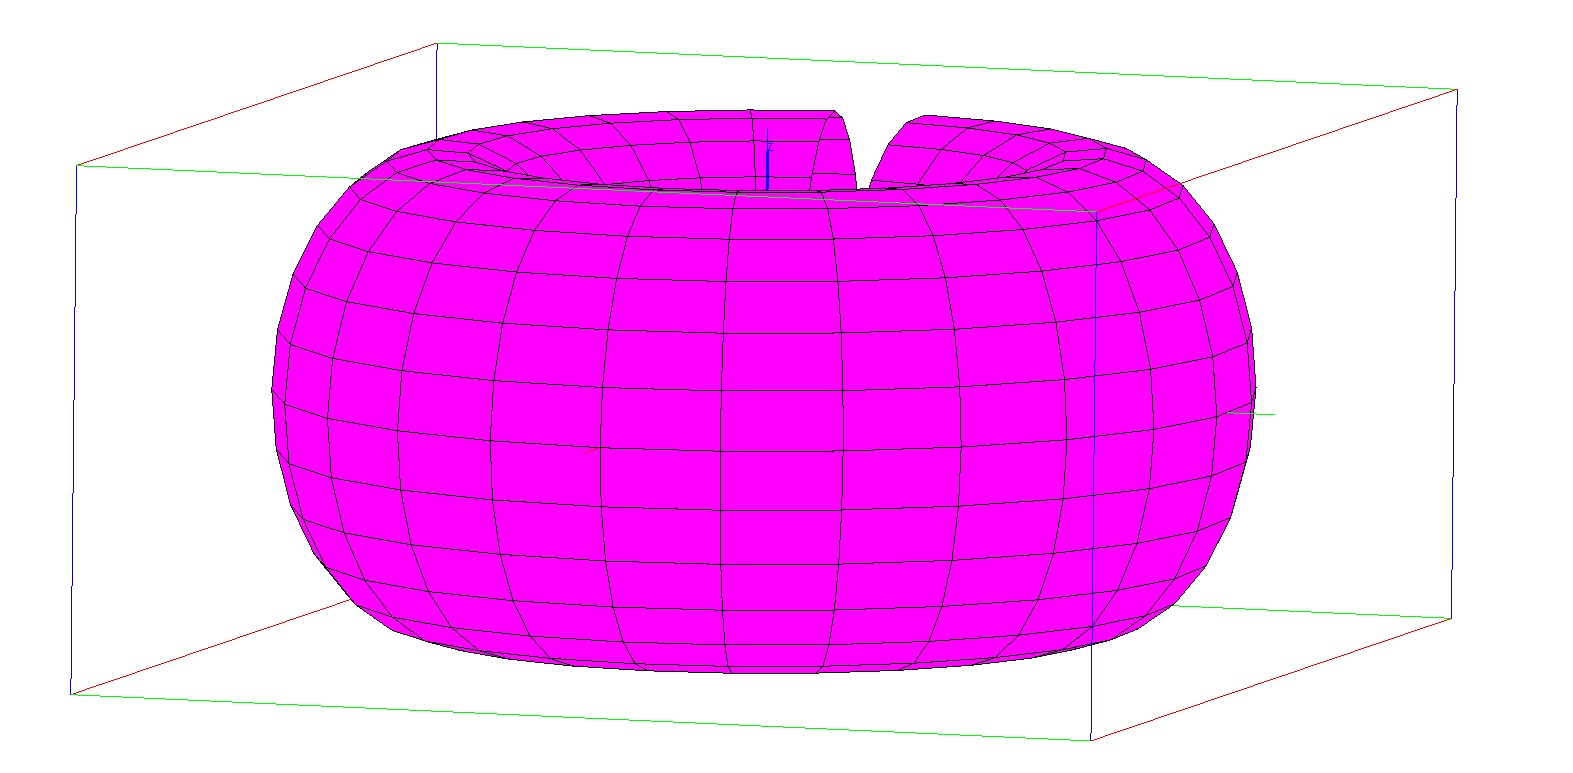
\includegraphics[scale=0.2]{ToreV3}
  \end{center}
\end{enigme}


%%% Local Variables:
%%% mode: latex
%%% TeX-master: "../Manuel-TS"
%%% End:

\end{document}